% $Id: template.tex 11 2007-04-03 22:25:53Z jpeltier $

%\documentclass{vgtc}                          % final (conference style)
%%\documentclass[review]{vgtc}                 % review
%%\documentclass[widereview]{vgtc}             % wide-spaced review
%%\documentclass[preprint]{vgtc}               % preprint
%%\documentclass[electronic]{vgtc}             % electronic version
%
%% Added by KM, 130928, to get it to compile. Not sure why.
%\let\ifpdf\relax
%
%
%%% Uncomment one of the lines above depending on where your paper is
%%% in the conference process. ``review'' and ``widereview'' are for review
%%% submission, ``preprint'' is for pre-publication, and the final version
%%% doesn't use a specific qualifier. Further, ``electronic'' includes
%%% hyperreferences for more convenient online viewing.
%
%%% Please use one of the ``review'' options in combination with the
%%% assigned online id (see below) ONLY if your paper uses a double blind
%%% review process. Some conferences, like IEEE Vis and InfoVis, have NOT
%%% in the past.
%
%%% Figures should be in CMYK or Grey scale format, otherwise, colour 
%%% shifting may occur during the printing process.
%
%%% These three lines bring in essential packages: ``mathptmx'' for Type 1 
%%% typefaces, ``graphicx'' for inclusion of EPS figures. and ``times''
%%% for proper handling of the times font family.
%
%\usepackage{mathptmx}
%\usepackage{graphicx}
%\usepackage{times}
%
%% K additions (commenting)
%\usepackage{xcolor}
%%\usepackage{pdfcomment}
%
%%% We encourage the use of mathptmx for consistent usage of times font
%%% throughout the proceedings. However, if you encounter conflicts
%%% with other math-related packages, you may want to disable it.
%
%%% If you are submitting a paper to a conference for review with a double
%%% blind reviewing process, please replace the value ``0'' below with your
%%% OnlineID. Otherwise, you may safely leave it at ``0''.
%\onlineid{0}
%
%%% declare the category of your paper, only shown in review mode
%\vgtccategory{Research}
%
%%% allow for this line if you want the electronic option to work properly
%\vgtcinsertpkg
%
%
%% sort citations
%\usepackage{cite}
%%\usepackage[sort]{natbib}
%
%
%%% =================================
%% inline comments[KM addition]
%\definecolor{DarkGreen}{rgb}{0.0, 0.6, 0.0}
%\definecolor{DarkRed}{rgb}{0.7, 0.2, 0.2}
%\definecolor{DarkMagenta}{rgb}{0.5, 0.0, 0.5}
%\definecolor{DarkCyan}{rgb}{0.0, 0.6, 0.6}
%
%%\newcommand{\inlinecomment}[3][]{$\lceil$\textbf{#1}~\textit{\textcolor{#2}{#3}}$\rfloor$}
%\newcommand{\inlinecomment}[3][]{\textbf{#1}~\textit{\textcolor{#2}{#3}}}
%
%\newcommand{\todo}[1]{\noindent \inlinecomment[TODO]{DarkRed}{#1}}
%\newcommand{\km}[1]{\noindent \inlinecomment{DarkGreen}{#1}}
%\newcommand{\ikComment}[1]{\noindent \inlinecomment[IK]{DarkCyan}{#1}}
%\newcommand{\bgComment}[1]{\noindent \inlinecomment[BG]{blue}{#1}}
%
%
%\newcommand{\kmEdit}[1]{\textcolor{DarkGreen}{#1}}
%% \newcommand{\grn}[1]{\textcolor{DarkGreen}{#1}}
%%% =================================
%
%

\chapter{Sketch: The Haptic Instrument}
\label{ch:hapticinstrument}


%% In preprint mode you may define your own headline.
%\preprinttext{To appear in an IEEE VGTC sponsored conference.}

%% Paper title.

%\title{Haptic Jazz: Designing Touch with the Haptic Instrument}
%\title{Improvising Design with a Haptic Instrument}

%% This is how authors are specified in the conference style

%% Author and Affiliation (single author).
%%\author{Roy G. Biv\thanks{e-mail: roy.g.biv@aol.com}}
%%\affiliation{\scriptsize Allied Widgets Research}

%% Author and Affiliation (multiple authors with single affiliations).
%%\author{Roy G. Biv\thanks{e-mail: roy.g.biv@aol.com} %
%%\and Ed Grimley\thanks{e-mail:ed.grimley@aol.com} %
%%\and Martha Stewart\thanks{e-mail:martha.stewart@marthastewart.com}}
%%\affiliation{\scriptsize Martha Stewart Enterprises \\ Microsoft Research}

%% Author and Affiliation (multiple authors with multiple affiliations)
\author{Oliver S. Schneider\thanks{e-mail: oschneid@cs.ubc.ca} \qquad \qquad Karon E. MacLean\thanks{e-mail: maclean@cs.ubc.ca}\\ %
        \scriptsize Department of Computer Science \\
        \scriptsize University of British Columbia, Vancouver, Canada
}
%\author{Oliver S. Schneider\thanks{e-mail: oschneid@cs.ubc.ca}\\ %
%        \scriptsize University of British Columbia %
%\and Karon E. MacLean \thanks{e-mail: maclean@cs.ubc.ca}\\ %
%        \scriptsize University of British Columbia %
%%\and Martha Stewart\thanks{e-mail:martha.stewart@marthastewart.com}\\ %
%%     \parbox{1.4in}{\scriptsize \centering Martha Stewart Enterprises \\ Microsoft Research}
%}

%% A teaser figure can be included as follows, but is not recommended since
%% the space is now taken up by a full width abstract.
%\teaser{
%  \includegraphics[width=1.5in]{sample.eps}
%  \caption{Lookit! Lookit!}
%}

%%\abstract{
%% Designing haptic phenomena is increasingly important but difficult.
%As the need to deploy informative, expressive haptic phenomena in consumer devices gains momentum, the inadequacy of current design tools is becoming more critically obstructive.
%%However, this increased activity  also makes it possible to characterize issues, and address them with advances in software engineering.
%%Designers face two primary obstacles.
%Current tools do not support collaboration or serendipitous exploration.
%Collaboration is critical,
%but direct means of sharing haptic sensations are limited,
%and the absence of unifying conceptual models for working with haptic sensations further restricts communication between designers and stakeholders.
%%Because there are no unifying conceptual models for working with haptic sensations, there are major communication problems between designers and stakeholders.
%%: neither designers, nor managers, nor users can articulate what they experience.
%%This is especially troublesome when designing pleasant, affective interactions that rely upon user experience.
%This is especially troublesome for pleasurable, affectively targeted interactions that rely on 
%subjective user experience.
%%In this paper, we introduce our solution: the haptic instrument, analogous to a musical instrument, a new tool for real-time, collaborative manipulation of haptic sensations.
%In this paper, we introduce an alternative design approach
%inspired by musical instruments -- a new tool for real-time, collaborative manipulation of haptic sensations;
%and describe % the design of 
%a first example, mHIVE, a mobile Haptic Instrument for Vibrotactile Exploration.
%%, which allows both designers and users to express vibrotactile \km{(VT)} ideas with a simple touchscreen interface.
%Our qualitative study shows that mHIVE supports exploration and communication but
%requires additional visualization and recording capabilities for tweaking designs,
%and expands previous work on haptic language.
%%and reveals future research directions for both design tools and language.
%%}


%% ACM Computing Classification System (CCS). 
%% See <http://www.acm.org/class/1998/> for details.
%% The ``\CCScat'' command takes four arguments.
%
%\CCScatlist{
%  \CCScat{H.5.2}{Information Interfaces and Presentation (e.g., HCI)}{User Interfaces}{Haptic I/O}
%}

%% Copyright space is enabled by default as required by guidelines.
%% It is disabled by the 'review' option or via the following command:
% \nocopyrightspace

%%%%%%%%%%%%%%%%%%%%%%%%%%%%%%%%%%%%%%%%%%%%%%%%%%%%%%%%%%%%%%%%
%%%%%%%%%%%%%%%%%%%%%% START OF THE PAPER %%%%%%%%%%%%%%%%%%%%%%
%%%%%%%%%%%%%%%%%%%%%%%%%%%%%%%%%%%%%%%%%%%%%%%%%%%%%%%%%%%%%%%%%

% Make sure hyperref comes last of your loaded packages, 
% to give it a fighting chance of not being over-written, 
% since its job is to redefine many LaTeX commands.
%\usepackage[pdftex]{hyperref}
%\hypersetup{
%pdftitle={SIGCHI Conference Proceedings Format},
%pdfauthor={LaTeX},
%pdfkeywords={SIGCHI, proceedings, archival format},
%bookmarksnumbered,
%pdfstartview={FitH},
%colorlinks,
%citecolor=black,
%filecolor=black,
%linkcolor=black,
%urlcolor=black,
%breaklinks=true,
%}


%Set graphics path

%% create a shortcut to typeset table headings
%\newcommand\tabhead[1]{\small\textbf{#1}}
%
%%new command that is a bold item
\newcommand\strongitem[1]{{\textbf{#1.}}}
%
%%new command that describes a theme:
\newcounter{themecounter}
\stepcounter{themecounter}
%%\newcommand\theme[1]{\vspace{2mm}\textbf{Theme \thethemecounter: #1}\stepcounter{themecounter}}
%%\newcommand\theme[1]{\subsection{Theme \thethemecounter: #1}\stepcounter{themecounter}}
\newcommand\theme[1]{\subsection{#1}}

%quote commands
\newcommand\q[1]{\textit{``#1"}} 			%\q for quote
\newcommand\sq[1]{{\q{#1}}}			%\sq for small quote
\newcommand\namedquote[2]{{\q{#2} (#1)}}
%\newcommand\namedquote[2]{{\textbf{#1:} \q{#2}}}
\newcommand\nq[2]{\namedquote{P#1}{#2}}	%\nq for named quote of participant number N
\newcommand\term[1]{\textit{#1}} 			%\term

%\numberofauthors{1}
%%\author{
%%  \alignauthor Author(s) Name(s)\\
%%    \affaddr{Affiliation(s)}\\
%%    \affaddr{Address(es)}\\
%%    \email{e-mail address(es)}\\
%%    \affaddr{Optional phone number(s)}
%%}
%
%
%%\keywords{
%%	vibrotactile; design tools;
%%	\textcolor{red}{Mandatory section to be included in your final version.}
%%}
%
%%\category{H.5.m.}{Information Interfaces and Presentation (e.g. HCI)}{Miscellaneous}
%%See: \url{http://www.acm.org/about/class/1998/}
%%for more information and the full list of ACM classifiers
%%and descriptors.
%
%\begin{document}
%% The ``\maketitle'' command must be the first command after the
%% ``\begin{document}'' command. It prepares and prints the title block.

%% the only exception to this rule is the \firstsection command

%%%%%%%%%%%%%%%%%%
%
% SECTION: Introduction
% 
%%%%%%%%%%%%%%%%%%
%\section{Introduction}

%%\maketitle
%
%Haptic feedback has hit %devices  are hitting 
%the mainstream, present in smartphones, gaming and automobile design,
%%Everything from smartphones to cars are adopting higher-fidelity haptic technology.
%but our knowledge of how to design haptic phenomena remains limited.
%%Despite years of research
%There are still no agreed-upon vocabularies or conceptual models for haptic phenomena \cite{Enriquez2003,Ledo2012,Lee2009,Obrist2013}, % putting \km{us} % haptic design at a loss when compared 
%in contrast to other modalities (\emph{e.g.}, using theory of minor chords to evoke a sad emotion in music).
%% Prospects are even more limited when developing sensations to have qualitative features, such as pleasant alerts or frightening game environments.
%For subjective qualities, such as pleasant alerts or frightening game environments, prospects are even more limited.
%%
%Design is still based on trial and error with programming languages, limiting exploration.
%%Programming languages are primarily used, limiting exploration.
%The lack of established conceptual models or design frameworks further challenges communication between designers and stakeholders.
%%The subset of tactile sensations has a number of candidates (e.g., vibrotactile score \cite{Lee2009}), but even this area can be improved.
%%In particular, existing tools fail to support designers in two ways:
%
%%\begin{itemize}
%%	\item Development cycles are still based on compile, run, adjust cycles, or hardware vendor demos/examples
%%	\item There is no understood mental model or design theory when creating haptic phenomena
%%\end{itemize}
%

%\begin{figure}[th] %  figure placement: here, top, bottom, or page
%   \centering
%   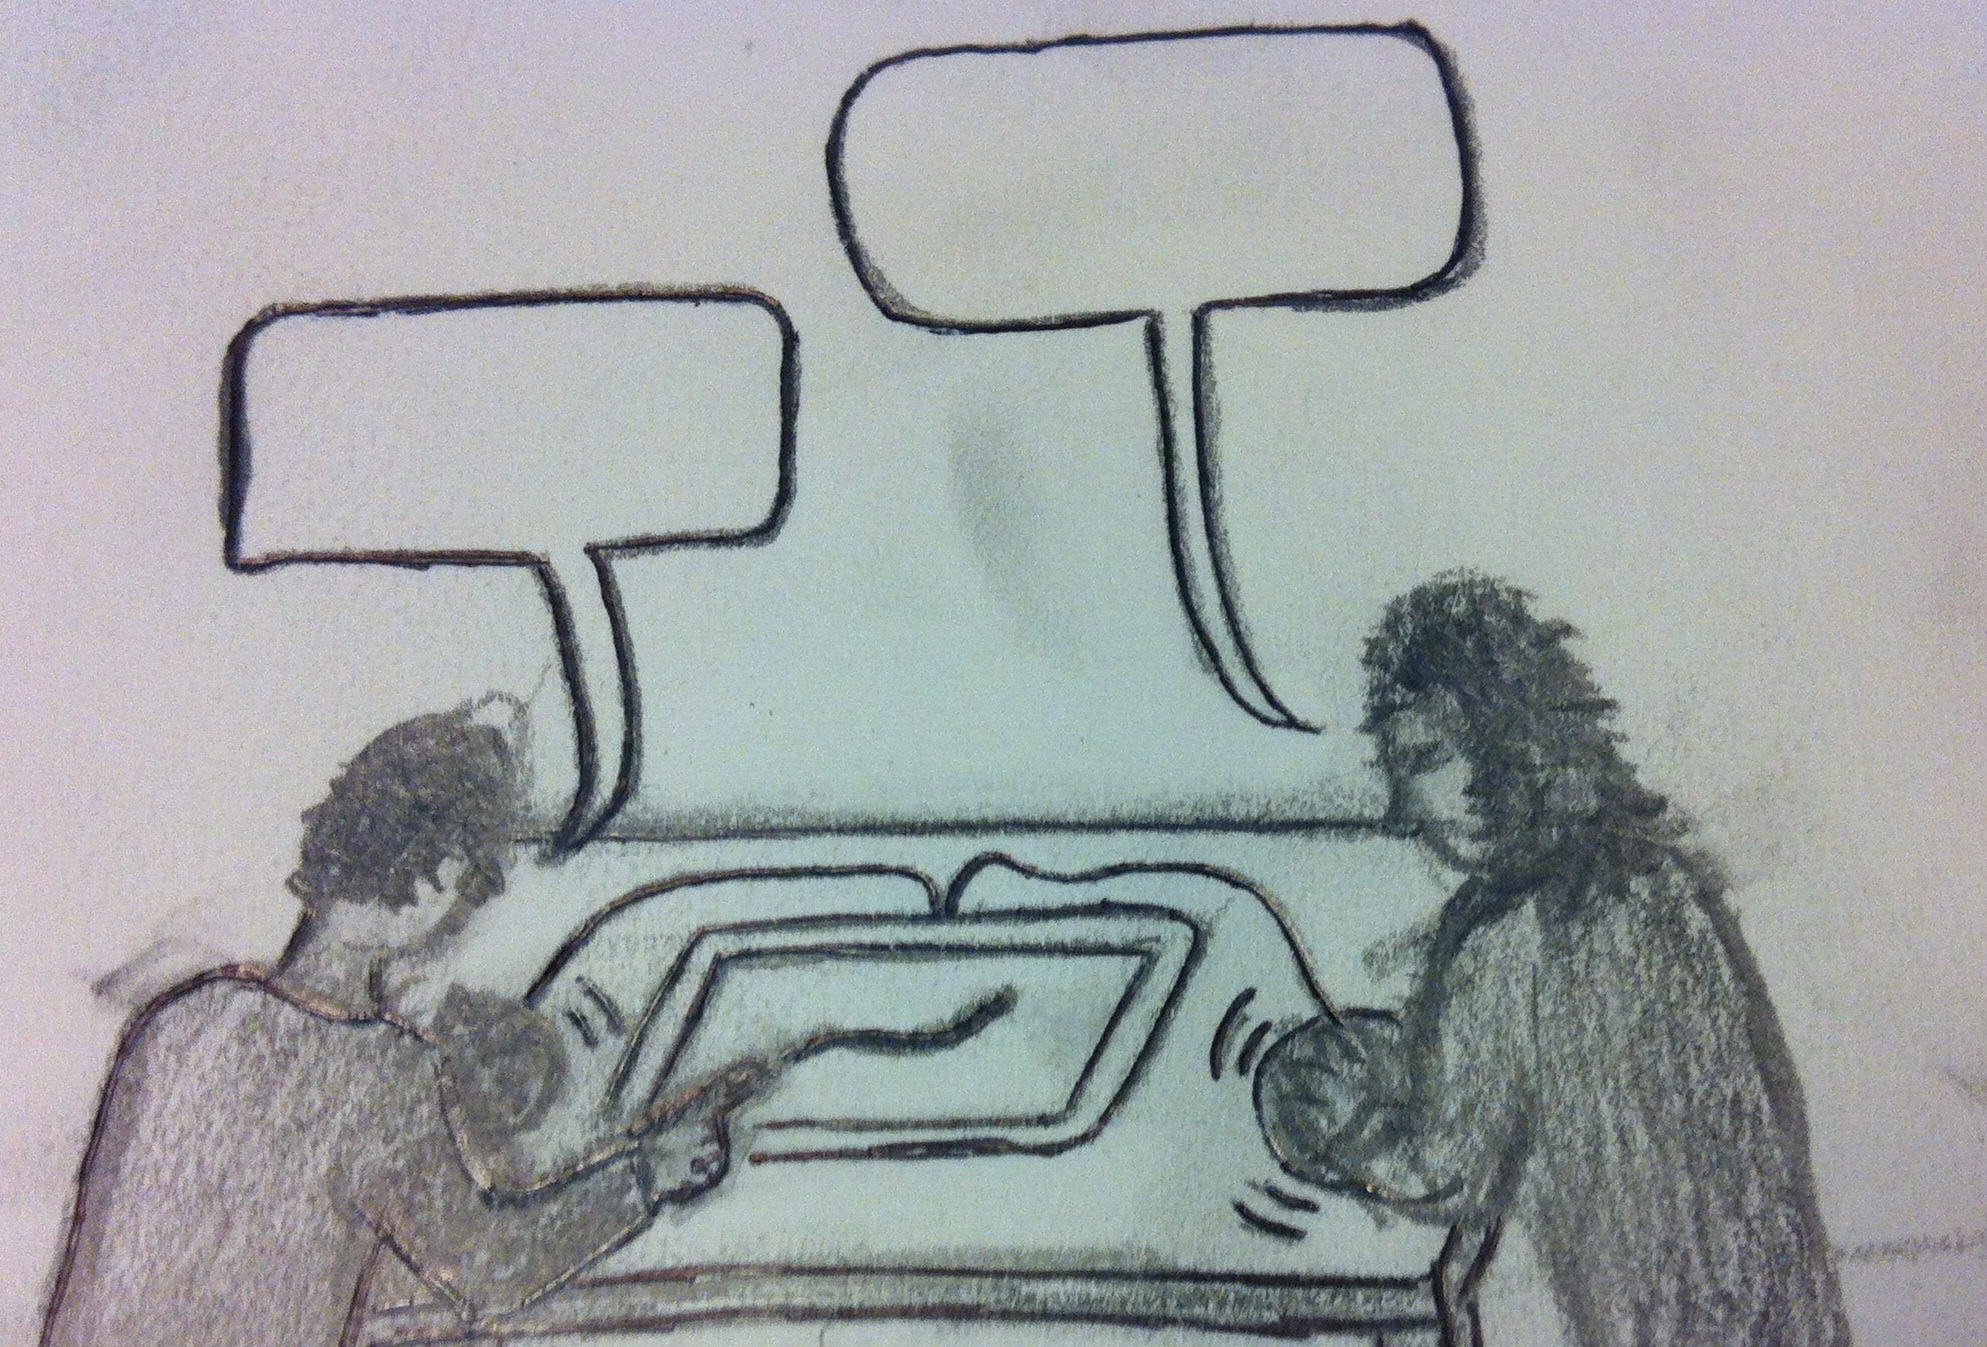
\includegraphics[width=0.4\textwidth]{HapticInstrumentConceptSketchRough} 
%   \caption{Concept Sketch of the Haptic Instrument}
%   \label{fig:HapticInstrumentConceptSketch}
%\end{figure}

\begin{figure}[h] %  figure placement: here, top, bottom, or page
   \centering
   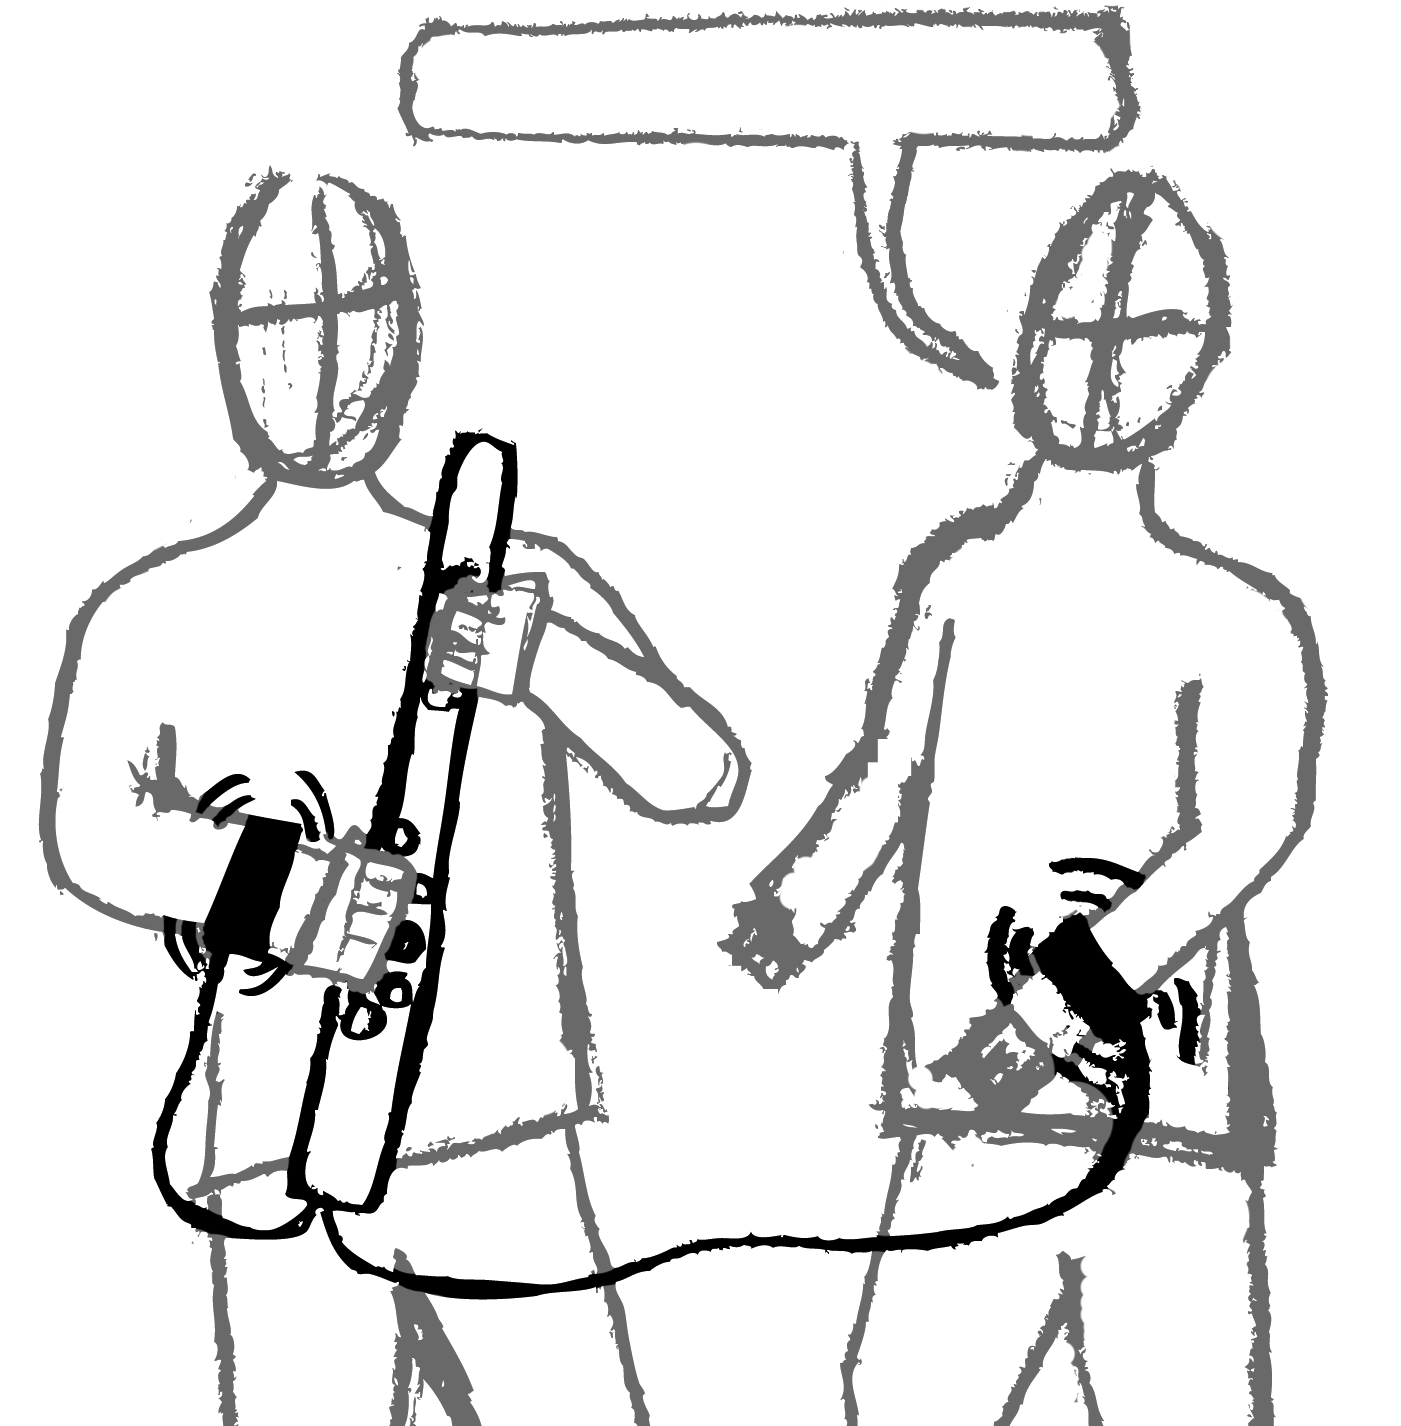
\includegraphics[width=0.5\textwidth, height=2.3in]{haptic-instrument-concept-sketch-sax-small-traced-squarer} 
   \caption{Concept sketch of a haptic instrument. Both users experience the same sensation, controlled in real-time.}
   \label{fig:HapticInstrumentConceptSketch}
\end{figure}

The Haptic Instrument case study\footnote{Published in Haptics Symposium 2014 \cite{Schneider2014} and at a CHI 2014 workshop \cite{Schneider2014b}.} is a first exploration into building a vibrotactile design tool, looking at design activities of exploration and informal sharing.
Through it, we investigate the role of real-time feedback and synchronous collaboration on haptic experience design, using participants with some haptics experience, serving as proxies for haptic experience designers.
Conventional haptic design tools contain a slow iteration, requiring programming or rendering before playback.
Using a music composition metaphor (as in~\cite{Lee2009}), we are writing music without ever playing a note: composing a work in its entirety, then listening to the result before making changes.
In contrast, musicians often use their instruments as a tool for serendipitous exploration when designing music.
%and can draw upon musical theory.
Furthermore, music is collaborative, with communication facilitated by a reference point of a sound.
%Touch, however, is a personal, local sense, making it difficult to discuss stimuli.


%Facilitated exploration and collaboration % in haptic design should 
%should streamline the haptic design process and inform a guiding 
%theory, analogous to those for musical composition. % theory. % vague?
%% With eased exploration, 
%Designers will attain fluency with new devices and control parameters,
%while collaborative elements % should help communication, but also 
%% could prove key to developing this theory.
%%Previous approaches have all been single-user design tools.
%%We suspect that adding a collaborative element is the key to developing these languages
%will get people designing in groups.  A usable haptic language may emerge from their dialogue.
%% they use to collaborate might emerge naturally from the collaborative interactions.


%Furthermore, recent work has identified major communication barriers in industry. Designers of haptic sensations are forced to carry examples of different textures or dynamical systems to make their point to stakeholders.



Our approach is to directly use a \emph{haptic instrument}, inspired by musical instruments but producing (for example) vibrotactile (VT) sensations rather than sound (\autoref{fig:HapticInstrumentConceptSketch}).
Haptic instruments are intended to have two main uses: they provide real-time feedback to the user to facilitate improvisation and exploration, and produce haptic output to multiple users as a \emph{what-you-feel-is-what-I-feel} (WYFIWIF) interface.
This allows for a dialogue that includes a haptic modality: haptic instruments create a shared experience of touch, allowing for a common reference point.


% when two or more people are talking.
%We hope that haptic instruments will not only prove to be useful tools in their own right, but also allow for a haptic language to emerge naturally from the dialogue surrounding this shared experience.
%We developed a vibrotactile instance, mHIVE (mobile Haptic Instrument for Vibrotactile Exploration), as a platform to investigate this concept.


%Our main contributions are:
%\begin {itemize}
%	\item A definition of the haptic instrument concept \& design space.
%	\item A fully-working haptic instrument (mHIVE).
%	\item The novel application of an established psychological methodology, phenomenology, to investigate mHIVE's interface and subjective tactile experiences.
%%	rather than psychophysical thresholds.
%	\item Preliminary results from a qualitative study that show mHIVE supports exploration and collaboration, and implications for the design of future haptic design tools.
%\end{itemize}

%%\noindent
%In this paper, we first cover the related work of haptic design tools and haptic language,
%%, identifying the progress so far in haptic design tools and conceptual models.
% then define the haptic instrument, its requirements, features, and design space.
%We report the design of mHIVE,
%% and the feedback we have encountered.
%our methodology, and preliminary results, and
%% investigating both the experience of using mHIVE and the language used to describe haptic phenomena.
% conclude with future directions for haptic tool design and research into a haptic language.
%%, and a vision for how haptic instruments can be used to develop a conceptual framework, the analogous musical theory for haptic sensations.
%%
%%\begin{itemize}
%%	\item Haptic jazz is a rich metaphor
%%	\item Haptic ``lead sheets" instead of scores
%%	\item improvisation
%%	\item social
%%\end{itemize}

\begin{figure*}[Htb]
   \centering
   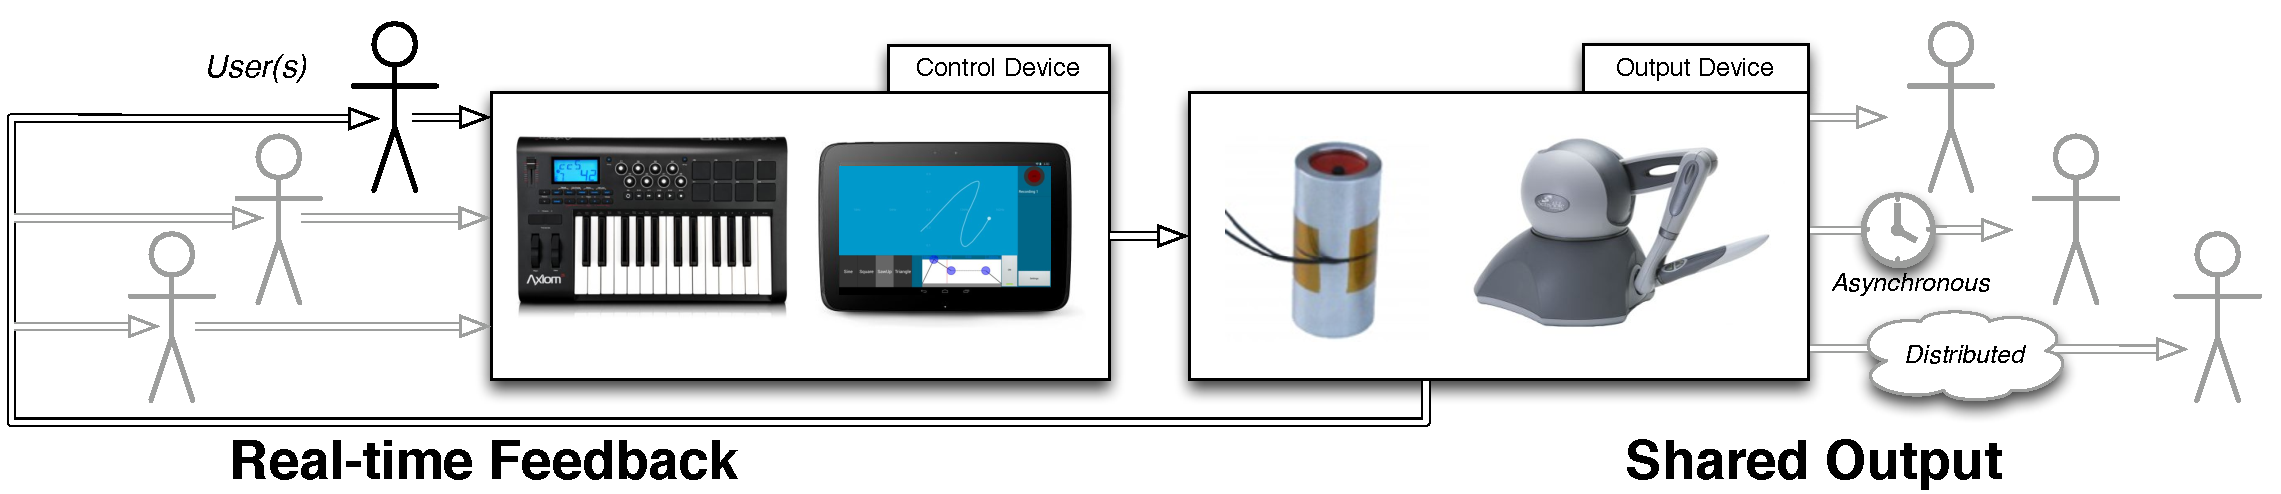
\includegraphics[width=\textwidth]{haptic-instrument-concept-horizontal4-small} 
   \caption{The haptic instrument concept. One or more people control the instrument, and receive real-time feedback from the device. Any number of audience members can feel the output in real time as well. Control methods can vary, from traditional musical control devices (such as the M-Audio Axiom 25, used in preliminary prototypes) to touchscreen tablets (used in mHIVE). Output devices vary as well.}
   \label{fig:HapticInstrumentConcept}
\end{figure*}




%Finally, we draw inspiration the Logo, which uses the ``transitionary object" of a turtle \cite{Papert1980}??? to aid users in making  to communicate experience, live coding ? Programming by example, haptic camera line of thought?


%%%%%%%%%%%%%%%%%%
%
% SECTION: Defining the Haptic Instrument
% 
%%%%%%%%%%%%%%%%%%
%\section{Defining the Haptic Instrument}
%We define a haptic instrument as a tool for general manipulation of one or more haptic (tactile, force-feedback, or both) devices that provides real-time feedback to anyone controlling the device, and can produce identical shared (WYFIWIF) output to all users to facilitate discussion and collaboration.
%Manipulation can include ideation, exploration, communication, recording, refinement, and articulation.
%Manipulation can be for utilitarian purposes (\emph{e.g.}, designing haptic notifications) or artistic expression (\emph{e.g.}, a haptic performance).
%Output devices can be purely output, or interactive.
%Furthermore, although haptic devices must be involved, multimodal experiences could easily be created by combining a haptic instrument with auditory or visual output.\footnote{One could even imagine a multimodal instrument such as Asimov's Visi-Sonor \cite{Asimov-Foundation-and-Empire} or its parody, Futurama's Holophonor \cite{Futurama-33-ParasitesLost}.}


%\begin{figure*}[htb]
%   \centering
%   \begin{minipage}{0.65\textwidth}
%	   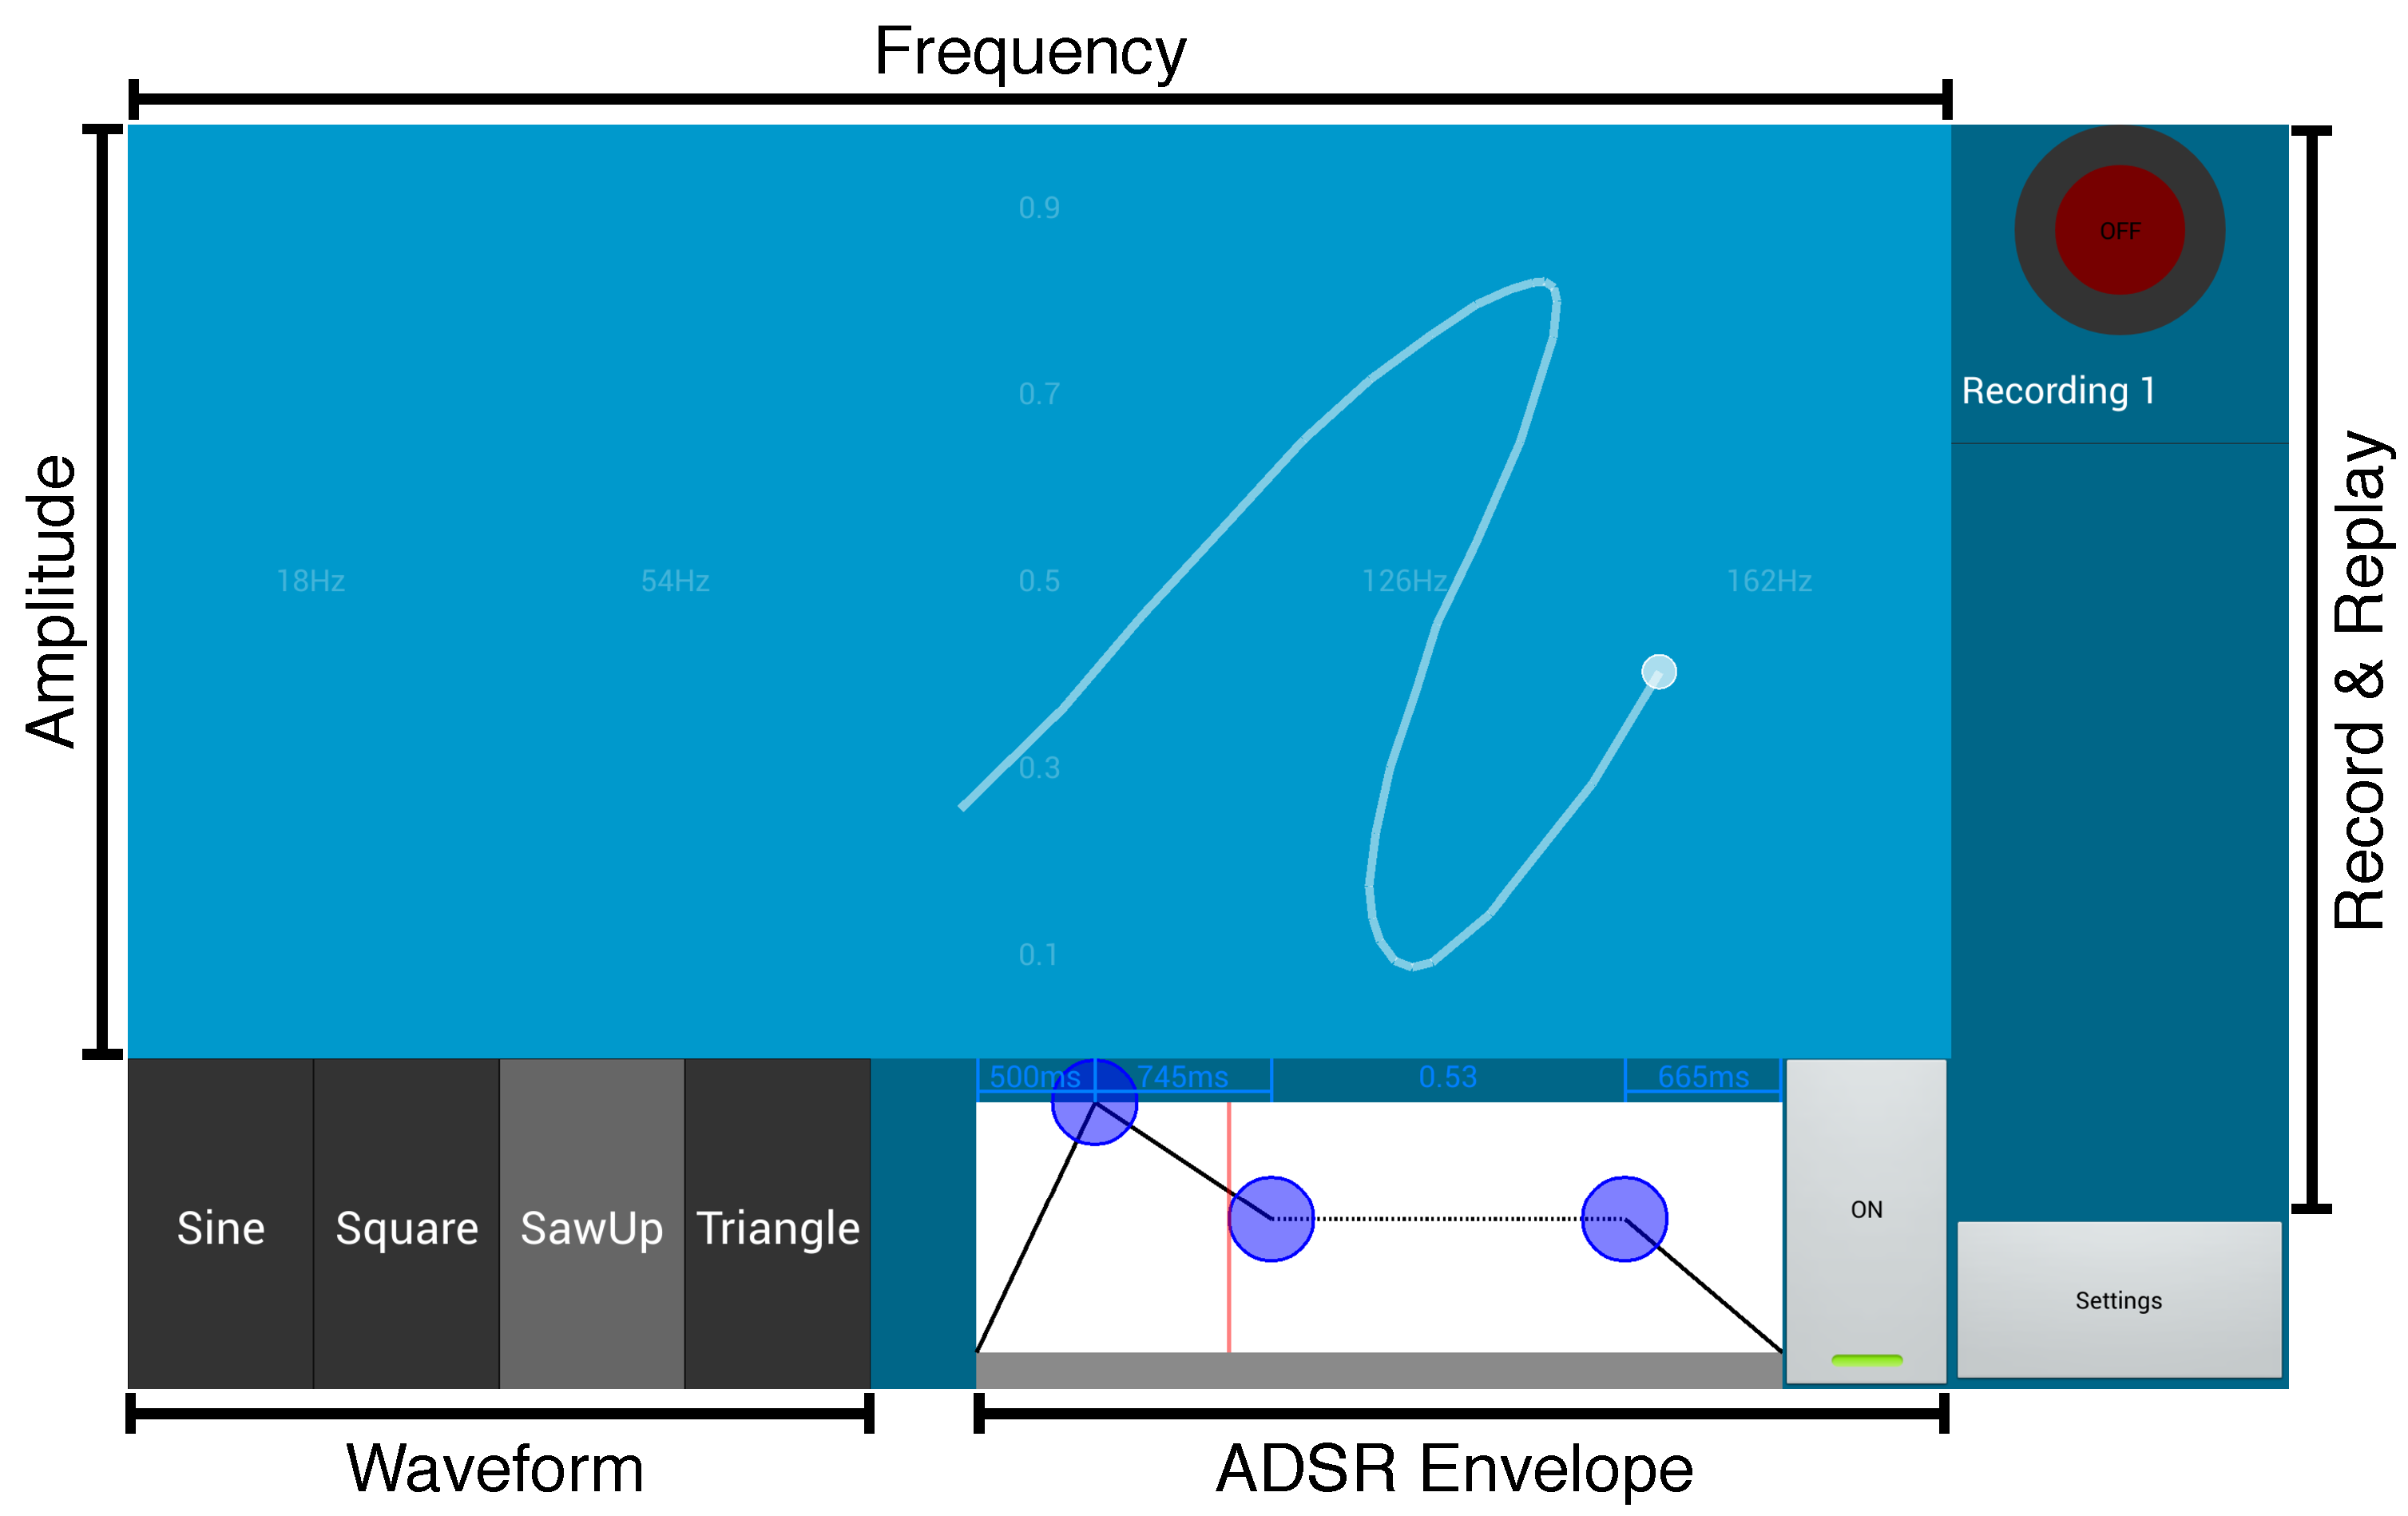
\includegraphics[width=\textwidth]{mHIVE-screenshot-labeled-2013-08-13} 
%	   \caption{mHIVE interface. Primary interaction is through the amplitude-frequency view, where visual feedback is provided through a circle (current finger position) and a trail (two seconds of previous interaction history).}
%	   \label{fig:mHIVE}
%    \end{minipage}
%    \hspace{1cm}
%   \begin{minipage}{0.25\textwidth}
%	   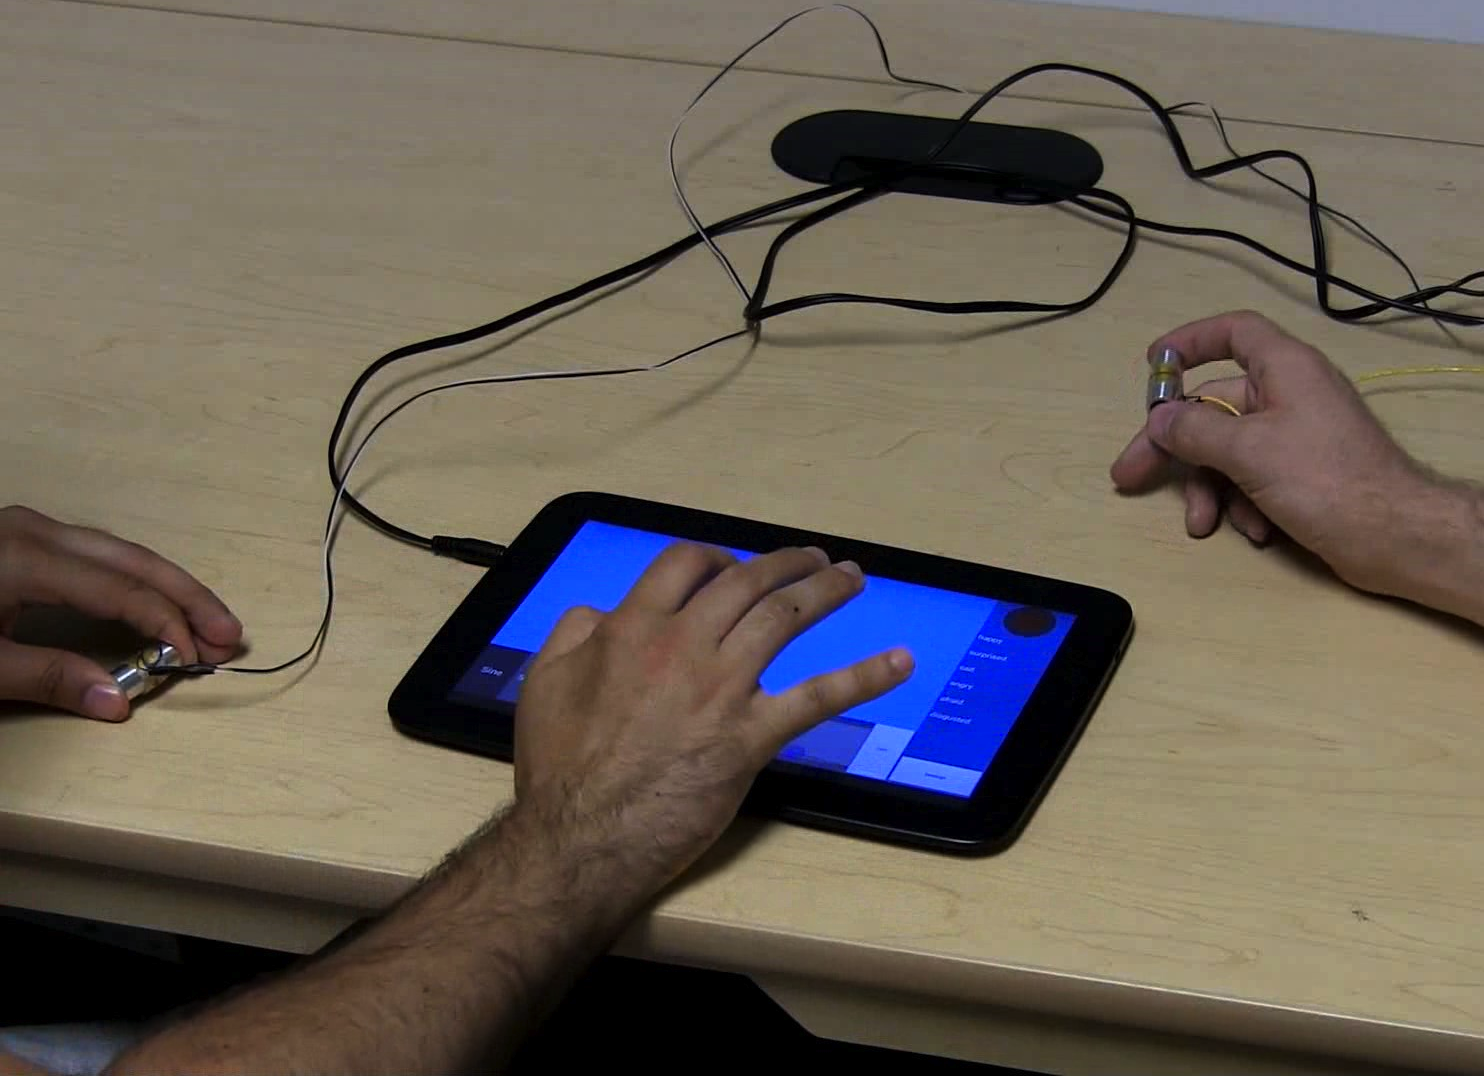
\includegraphics[width=\textwidth]{mHIVE-study-setup-cropped} 
%	   \caption{Study setup. The participant (left) controls the device while feeling the sensation; the interviewer (right) feels the same sensation on an identical output device.}
%	   \label{fig:StudySetup}
%    \end{minipage}   
%\end{figure*}





%%%%%%%%%%%%%%%%%%
%
% SECTION: mHIVE
% 
%%%%%%%%%%%%%%%%%%
\section{Design}

%%%%%
%SubSection: Design Dimensions
%%%%
%\subsection{Design Dimensions}
%Though haptic instruments by definition provide real-time feedback have shared-output, there are several main design dimensions that can be considered in a haptic instrument (outlined in \autoref{fig:HapticInstrumentConcept}).
%Note that haptic instruments can occupy multiple positions on these dimensions.
% Though haptic instruments by definition provide real-time feedback \kmEdit{??} have shared-output, 
There are several main design dimensions that can be considered in a haptic instrument (outlined in \autoref{fig:HapticInstrumentConcept}).
A haptic instrument can occupy multiple positions on these dimensions.
%; a haptic instrument could allow for both synchronous and asynchronous collaboration.

%\begin{description}

	\strongitem{Asychronous/synchronous}
%	Because of the shared-output,
%A haptic instrument collaborative.
Though a haptic instrument must provide real-time feedback, its collaborative (shared-output) aspect could be either synchronous (by having multiple people experience the real-time output) or asynchronous (by allowing for recording and playback, important for design).
%Indeed, recording is critical when creating musical pieces.

	\strongitem{Collocated/distributed} A haptic instrument's output could be present only for users in the same room, or be broadcast over a network to people around the world. For example, multiple mobile devices could all display identical output in a distributed manner.

	\strongitem{Private/shared %KM suggested collaborative, not going with it because of our use of "collaborative" elsewhere
control} A haptic instrument's control % interface 
 could be private (operated by a one person at a time) or shared (multiple users control the display). 
Shared control could be collocated or distributed (\emph{e.g.}, a web interface and shared object model).
	
	\strongitem{Output mechanism} Each haptic instrument will control a haptic device, which has its own mechanism for providing a haptic sensation (\emph{e.g.}, vibrotactile sensations). Because haptic devices can be complex and combine multiple mechanisms, this is a large space in its own right. Characterizing the different display mechanisms is something that we must leave to future work. Suffice it to say, a haptic instrument will be different depending on its output device.

	\strongitem{Number of haptic instruments or output devices}
	One consideration is whether a haptic instrument is intended to operate alone, or with other haptic or multimodal instruments.
%	\kmEdit{slc} % Don't you need to mention also, multimodal design? jam the haptic channel along with the auditory?
	One can imagine haptic jam sessions for inspiration and ideation, or even form haptic bands for artistic expression.
	This is highly related to private/shared control -- there is a fine line between several identical haptic instruments with private control, and a single haptic instrument with shared control and several output devices. Note that a haptic instrument may involve several devices to produce shared-output.

	\strongitem{Control mechanism} Similarly, a haptic instrument could be controlled in a variety of ways.
	From musically-inspired MIDI controllers to smartphone applications, we envision a wide variety of control methods.
%	Even a real-time programming environment might be appropriate for complex interactive sensations.
%	One should note that the control mechanism must work with the output device's paradigm.
	Even a real-time programming environment might be appropriate for complex interactive sensations,
	so long as the control mechanism works with the output device's paradigm.
%	 likely depend on the display mechanism, as many display mechanisms required their own paradigm for control.

%\end{description}
%
%We expect that haptic instruments could provide both immediate and long-term value.
%% In the short term, 
%We hope haptic instruments will improve the design process immediately, by supporting exploration and collaboration.
%% won't just be valuable on their own, but might produce emergent value.
%%We also expect that there will be other valuable results that are emergent from.
%%We expect that exploration will help designers quickly internalize the meaning of different control parameters for a given device.
%%of different display mechanisms and the parallel differences in control paradigms.
%%Collaboration, on the other hand, could develop an explicit conceptual model or language analogous to musical theory that could aid haptic designers.
%Over time, their use could lead to a natural, emergent design language valuable in its own right.
%One can also imagine a general tool composed of several virtual haptic instruments, much like digital musical synthesizers.
%
%%User stories, requirements?

\begin{figure}[Htb]
   \centering
%	   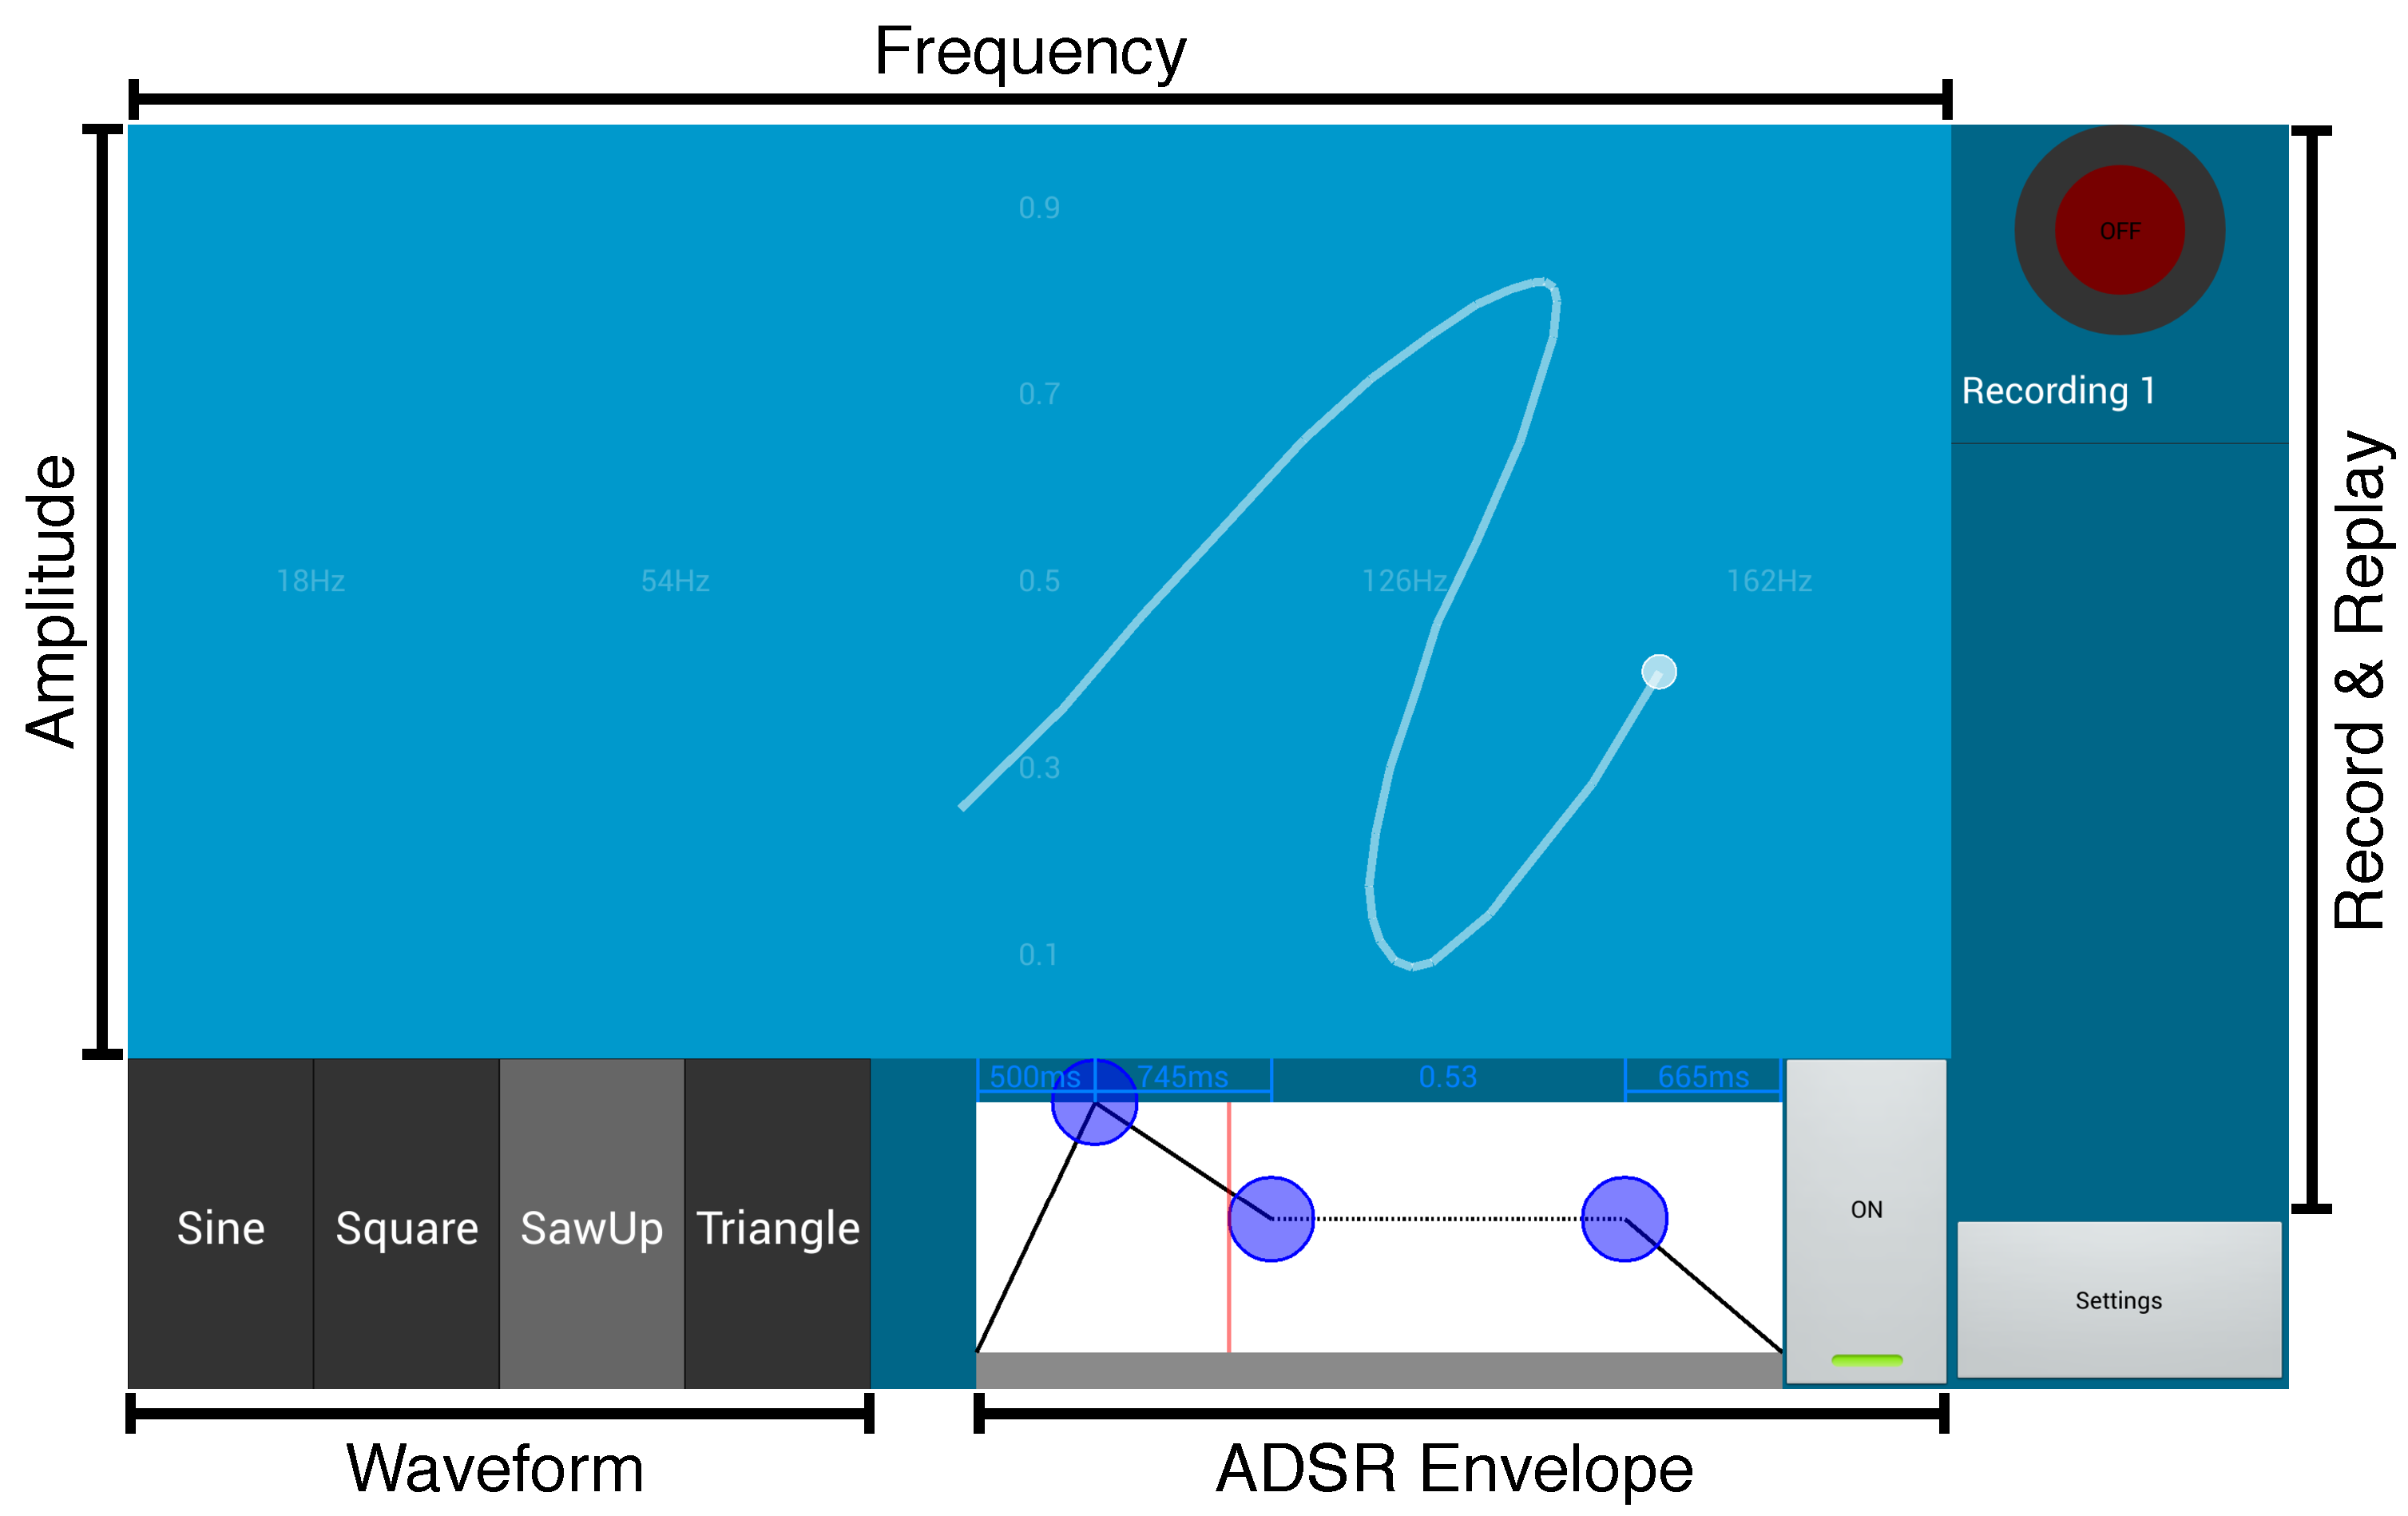
\includegraphics[width=0.43\textwidth]{mHIVE-screenshot-labeled-2013-08-13} 
	   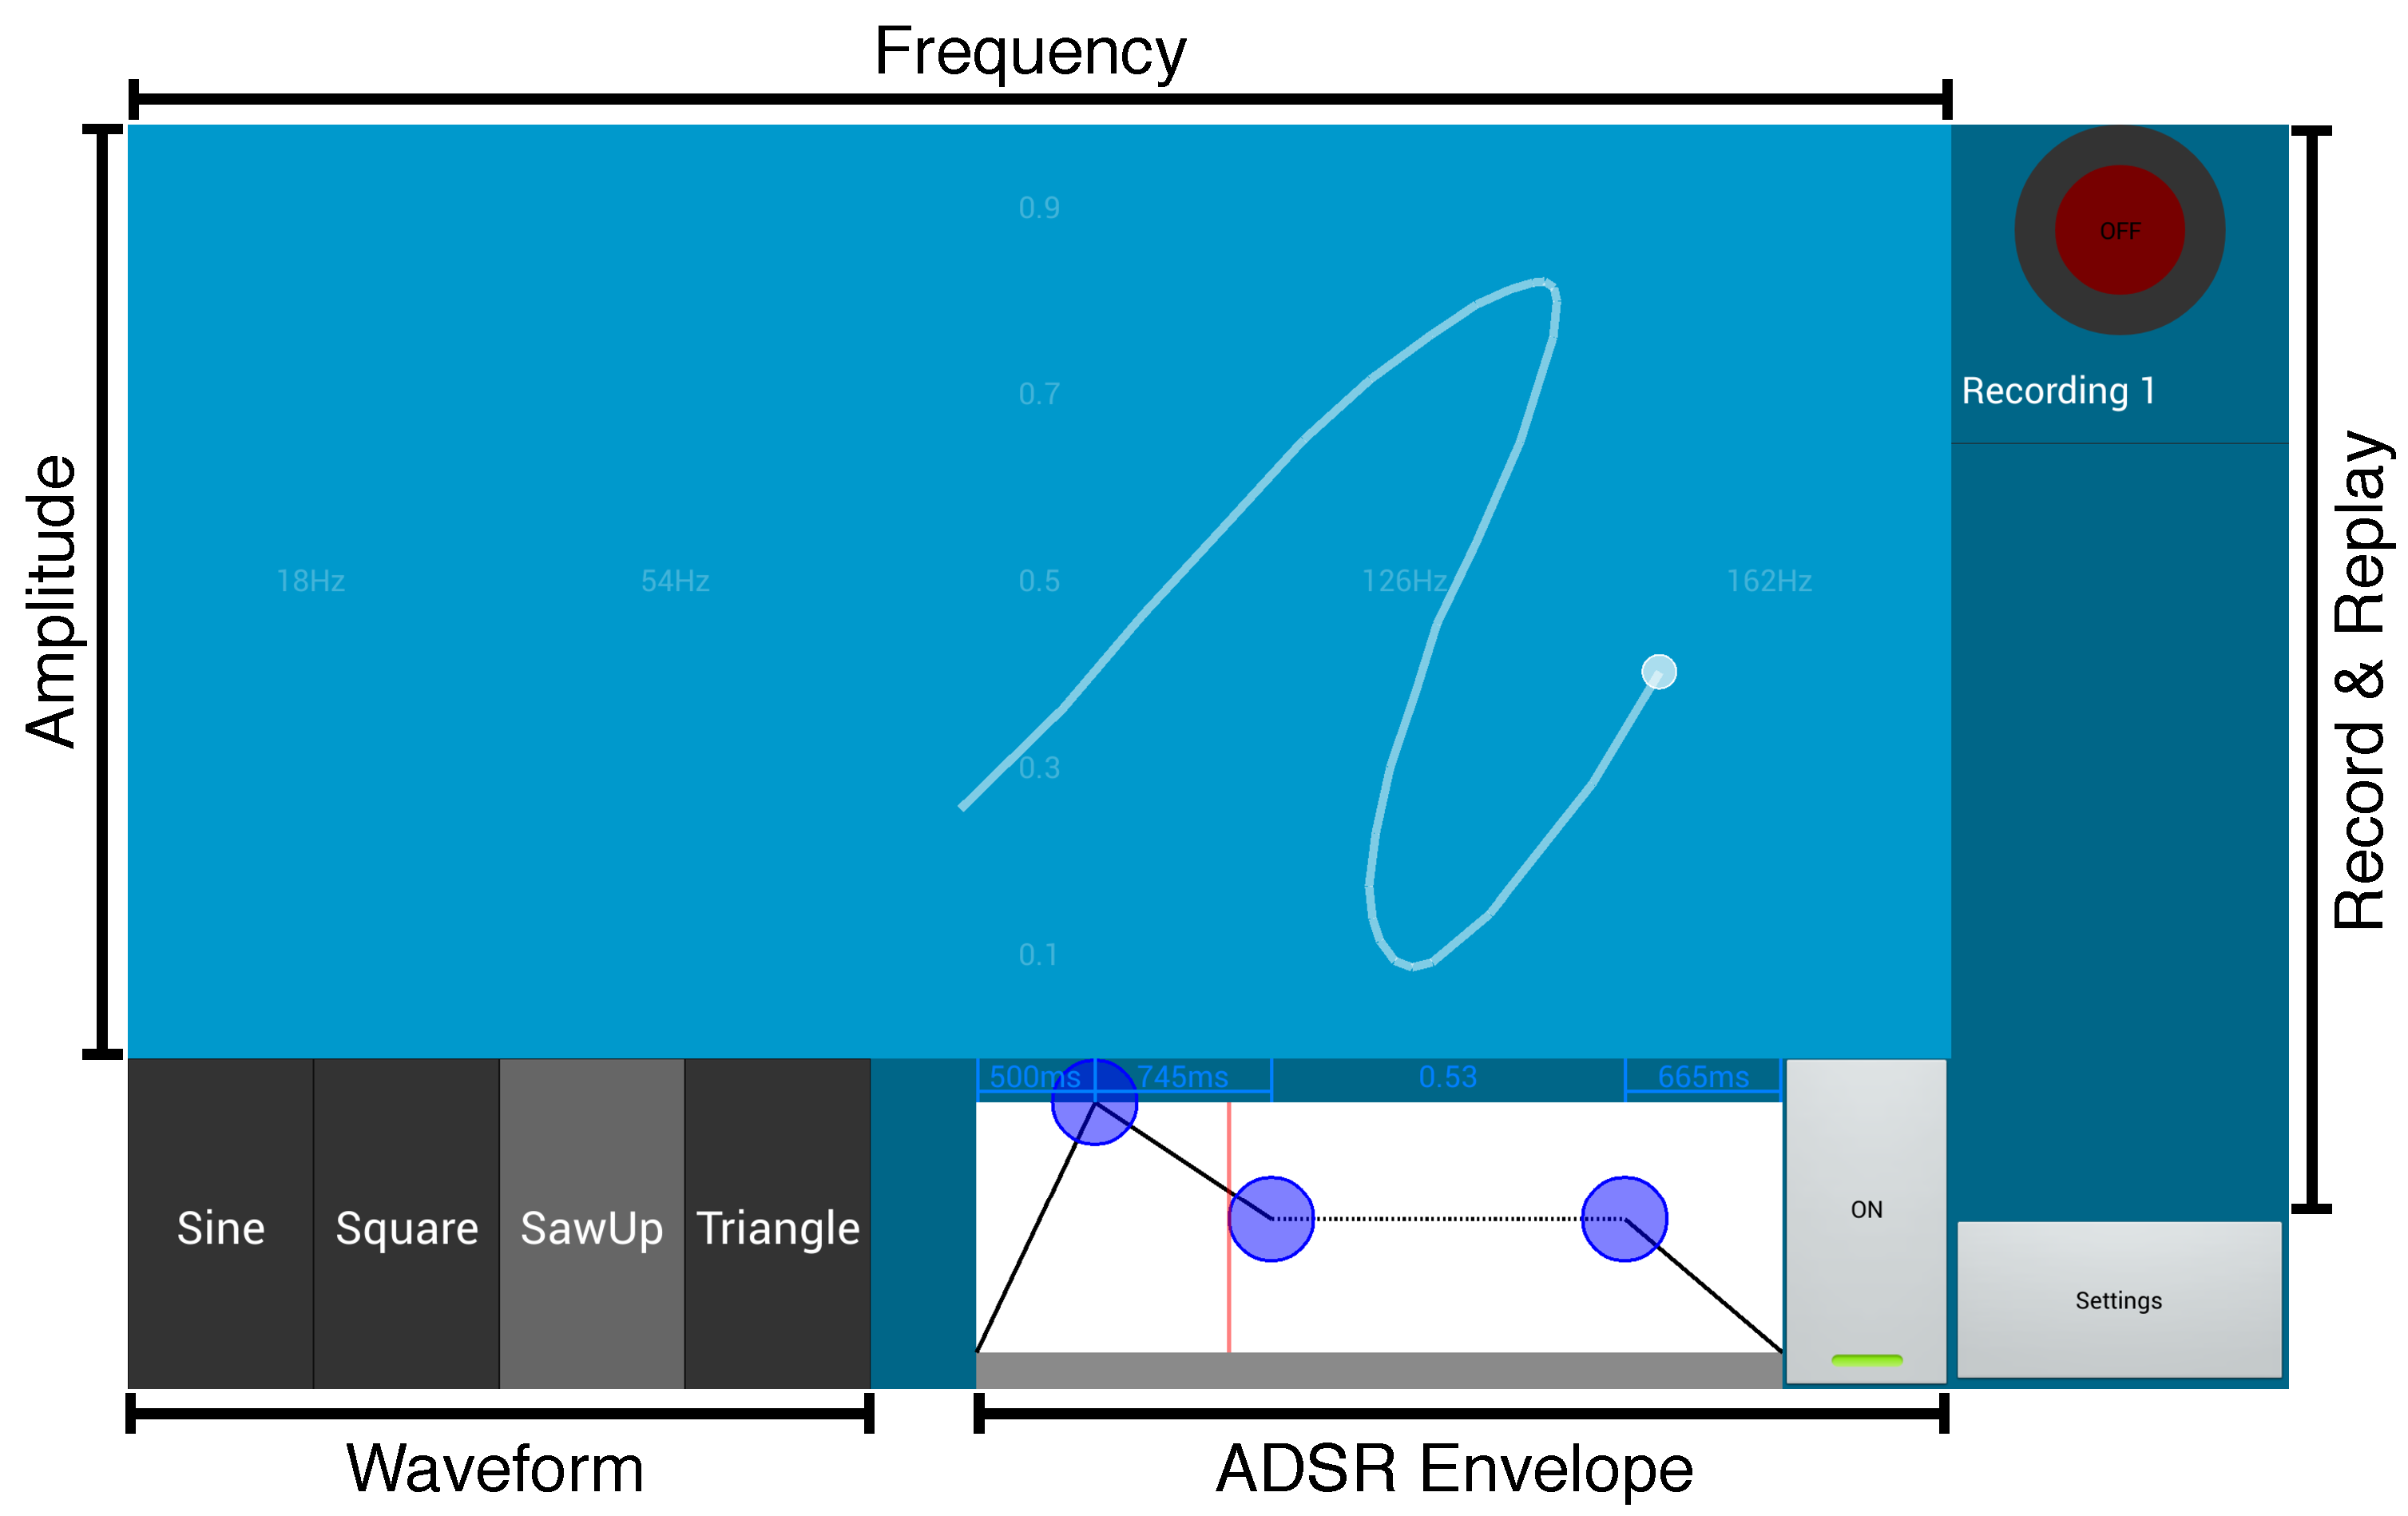
\includegraphics[width=0.7\textwidth]{mHIVE-screenshot-labeled-2013-08-13} 
	   \caption{mHIVE interface. Primary interaction is through the amplitude-frequency view, where visual feedback is provided through a circle (current finger position) and a trail (interaction history).}
	   \label{fig:mHIVE}
    \end{figure}



\subsection{mHIVE}%, a mobile Haptic Instrument for Vibrotactile Exploration}
We developed mHIVE, a mobile Haptic Instrument for Vibrotactile Exploration, to begin to explore how a haptic instrument should work and what it should do (\autoref{fig:mHIVE}).
% , we  developed a prototype, mHIVE (mobile Haptic Instrument for Vibrotactile Exploration,
%
%\footnote{Our first, low-fidelity prototype was named HIVE, before we switched to developing on a mobile platform. }
%
% mHIVE is a collocated, synchronous, mostly private control haptic instrument that controls 2 vibrotactile actuators
mHIVE is a collocated, synchronous haptic instrument for a single user. It accommodates shared display via dual
Haptuators~\cite{Yao2010}
and is operated with a single-touch tablet-based interface for direct manual control (\autoref{fig:hapticinstrument:StudySetup}). 
mHIVE is designed for for VT
% We chose this as a simple first attempt at a haptic instrument: vibrotactile 
sensations, which are common, do not require interactive programming, are controlled through waveforms (analogous to music), and their low-level control parameters are well understood.
%As well, they are commonly used in commercial devices, such as smartphones.
%Using a touchscreen % interface 
%allowed %was chosen for 
%direct manual control, similar to most musical instruments. % of the control parameters.
%: early desktop prototypes were awkward.



mHIVE offers real-time control of frequency, amplitude, waveform, envelope, duration, and rhythm, identified as the most important parameters for VT sensations \cite{Gunther2002,Brown2006a,Brown2006,Brewster2004, Rovan2000}.
mHIVE is implemented in Java using the Android SDK \cite{AndroidOpenSourceProject2012}, and the FMOD sound synthesis library \cite{fmod2013} to produce sounds, sent to two or more Haptuators through an audio jack.
%Thus, mHIVE is effectively a sound synthesizer designed for tactile sensations.
We deployed mHIVE on an Android Nexus 10 tablet running Android 4.2.1.



%mHIVE allows for control of frequency (5-180Hz, determined through piloting) and amplitude (0 (min) to 1 (full)) by drawing on a main input canvas.
%The ADSR filter can be toggled on or off by an adjacent button.
%As well, mHIVE allows for the user to record their input for later play back.
%Recording captures all input events, including waveform selection, ADSR manipulation, frequency/amplitude input, and even recording playback.

%%%%%%%%%%%%%%%%%%
%
% SECTION: Study Methodology
% 
%%%%%%%%%%%%%%%%%%
%\clearpage
\section{Study}

%%%%%%%%%%%%%%%%%%
%
% SECTION: Study Methodology
% 
%%%%%%%%%%%%%%%%%%
%\clearpage
% With mHIVE built, 
We conducted a qualitative study to investigate two questions.
%\km{Q1/Q2?slc} % consider numbering them for more structered reference later. gives a bit of formalism.
First, is mHIVE an effective tool for the expression, exploration, and communication of affective phenomena?
Second, what language, mental models, and metaphors do people use to describe vibrotactile sensations, and how do they relate to mHIVE's low-level control parameters?

\begin{figure}[Htb]
	\centering
%	   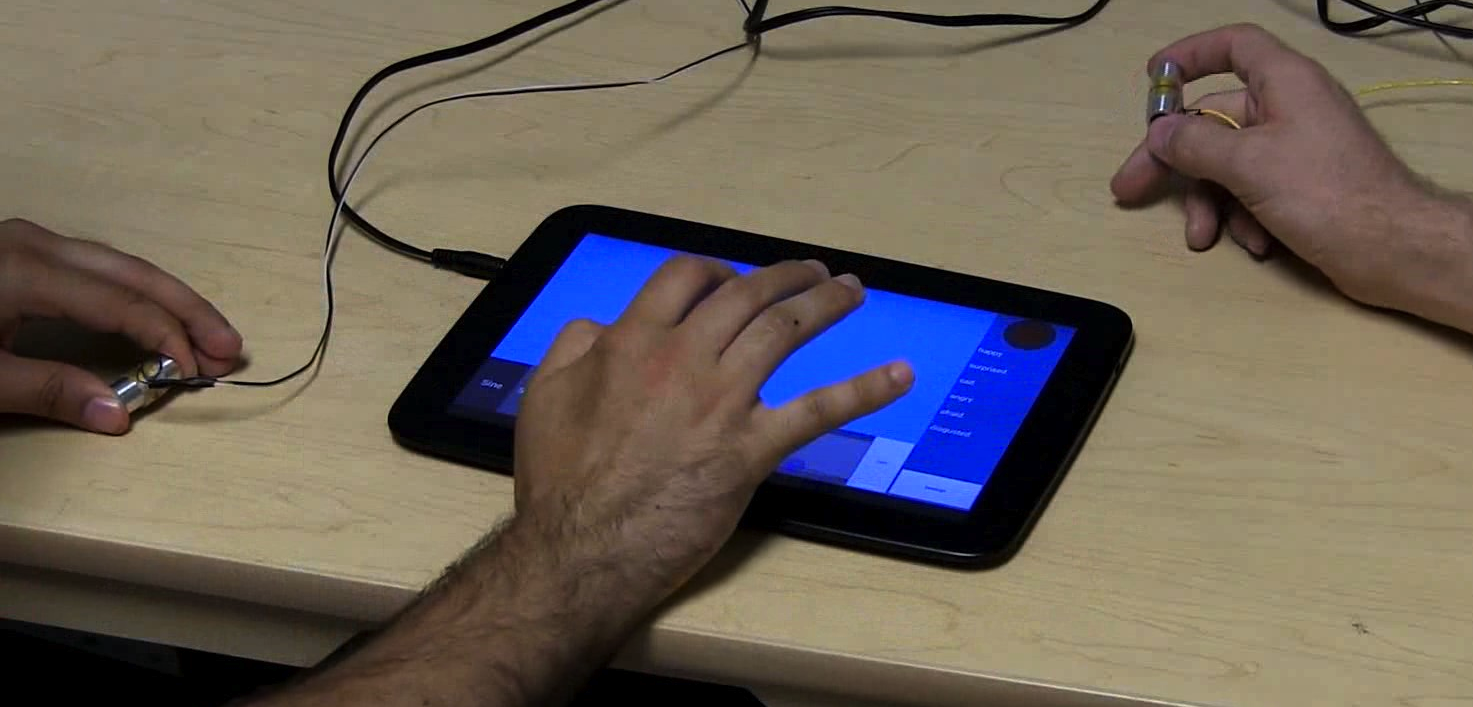
\includegraphics[width=0.32\textwidth]{mHIVE-study-setup-cropped2} 
	   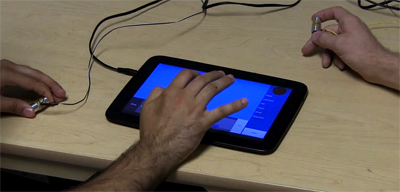
\includegraphics[width= 0.65\textwidth]{mHIVE-study-setup-cropped2small} 
	   \caption{
	   Study setup. Both the participant (left) and the interviewer (right) feel the same sensation as the participant controls mHIVE.
%	   The participant (left) controls mHIVE while feeling the sensation; the interviewer (right) feels the same sensation.
}
	   \label{fig:hapticinstrument:StudySetup}
\end{figure}

%\subsection{Procedure}
One researcher collected and analyzed data using the Stevick-Colaizzi-Keen method as described by Moustakas \cite{Moustakas1994}.
Our 1-hour open-ended interviews
%with four participants, all with haptic experience.
used the following protocol:
\begin{enumerate}
	\item Ask the participant for their background: occupation, experience with touchscreens, haptics, music, and video games.
	\item Demonstrate mHIVE to the user, and invite them to explore while thinking aloud to describe the sensations they feel.
	\item Probe the design space by asking participants to explore different control parameters, and to explore their metaphors (\emph{e.g.}, if the participant describes a sensation as ``smooth", R1 would ask them to try to produce a ``rough" sensation).
	\item Ask the participants to produce sensations for the six basic cross-cultural emotions documented by Ekman \cite{Ekman1992}, and rank how well they think their sensation represents the emotion on a 4-point semantic differential scale (Very Poorly, Somewhat Poorly, Somewhat Well, Well). This was done both as an elicitation device to gather a wider range of interactions with mHIVE, and to directly investigate a design task.
	\item Set the Haptuators down, and ask the participants to describe their experience of working with mHIVE in as complete detail as possible to evaluate the device itself.
\end{enumerate}

\noindent
R1 conducted the interviews and analysis, which required specialized knowledge of mHIVE.
%, and inductive nature of analysis did not allow for other researchers to cluster separately.
% Because clustering was conducted and not coding, 
%\kmEdit{Because we conducted clustering rather than coding,??}
Scores of inter-rater reliability common with other qualitative analyses (\emph{e.g.}, grounded theory \cite{Corbin2008}) are inappropriate and unavailable, as we did not conduct deductive, low-level coding.
To improve reliability,  R1's documented experience was analyzed first, and then consulted during analysis to remove bias (\emph{e.g.}, to not use terms only used by the experimenter).
%documented and analyzed his own experience with the device, which was considered when conducting analysis.
%we present here separately from other results to clearly demarcate the researcher's biases and preconceptions.
%Even so, results are grounded in empirical data, shown by quotations representing the clusters.
%Participants will also be contacted after analysis to provide feedback on our initial conclusions \textbf{TODO}.

%%%%%%%%%%%%%%%%%%
%
% SECTION: Results
% 
%%%%%%%%%%%%%%%%%%
\section{Results}

We sought participants with experience designing haptics as a proxy for expert designers for our initial study.
Four participants were recruited through email lists and word-of-mouth (P1-4, three male), and were all in the age range of 26-35 with self-reported occupations including graduate students or post-docs in information visualization, HCI, and human-robot interaction.
All had experience working with haptic technology, and (because of this requirement) all knew the main researcher in a professional capacity, although only P2 had seen earlier prototypes of the haptic instrument.
The small sample size, typical for phenomenological studies \cite{Creswell2013}, was appropriate for the rich data we wanted.
Data collection ended when we achieved saturation of new results, and had a clear direction for our next iteration.

%determined by saturation of new data: when we stopped encountering new data, we stopped recruiting participants.

%Analysis revealed several themes among the participants, particularly about the device's role in the design process, a tendency towards audio metaphors or concrete example-based metaphors, and a notion of enjoyable sensations vs. non-enjoyable sensations.
%As well, usability concerns are reported, suggesting implications for the design of future haptic instruments.

%
% Subsection: Reflections
%
%\subsection{Researcher Reflections and Experience}

%\emph{Note: This section is written by the researcher who led development of mHIVE and conducted the interviews and analysis.}

%%Researcher eval v1
%%As the principle developer of mHIVE, I have a unique outlook on the device.
%%I entered the study with planned improvements derived from piloting.
%%Deliberate exploration of the device revealed a number of takeaways which I will report here.
%%Some are may be similar to the experience reported by study participants, and some are specific to me.

%%Because I built the device, I understood the underlying mental model, and thus found mHIVE to be \q{very intuitive,} and \q{very helpful.}
%%I \q{enjoyed using it.}
%%I found visual trace and ADSR envelope to be \q{helpful.}
%%In particular, ADSR was very \q{important} to me, and was useful to \q{soften the edges} of the sensations.

%%However, I do not believe that mHIVE is perfect.
%%First, the addition of multitouch is \q{important.}
%%I found it was tricky to \q{juggle both hands}, feeling the output while simultaneously controlling the interface.
%%I have mixed feelings about the recording feature. Though I found it \q{helpful the one time} when developing the surprise sensation, I only used it once and feel that it \q{needs work.}
%%I had originally though that the recording feature needed a stop button, but \q{I didn't used it enough to notice} any lack of such a feature.

%%Finally, I found myself changing waveform and ADSR infrequently; it was \q{easy to leave something in place.}
%%Overall, I felt that mHIVE was \q{an exploratory tool} rather than a tool for \q{refinement.}
%%It would be best suited to exporting icons to \q{another application or another task.}

%%researcher eval v2
%Because I built the app, I understood the underlying system model. Because of this, I enjoyed using it, thought it was helpful, and found it intuitive and easy-to-use. I thought visual trail was very nice and helpful, because I could see where it was, and that ADSR was important, especially for a ringing sensation. I experienced unexpected sensations, calling them weird.

%Of course, because I was using an early prototype, there were still some interface-level refinements I thought were important to make. Some of these became less important as I interacted with the device. I thought that it needed a button to stop replay, but because I only used the record/replay feature once when exploring the device and didn't notice the lack of a stop button, I thought it was fine. Interacting with the device, multitouch emerged as an important feature to try. Overall, I though mHIVE was suited for exploration but not refinement, and thought it might be a good idea to record haptic icons and export them to another application.

%Low frequency sensations stood out to me as oscillating, pushes, thumps or hits (with the square wave), and felt like a watch or subwoofer. I described some low-level sensations with onomatopoeias, including djoo djoo djoo, wub wub wub, tick tick tick tick. ADSR allowed sensations that felt like soft bells, and that made me picture the sound of an ocean swelling. I made frequent analogies to technology: lasers, boat motors revving, and zippers, and could hear higher frequencies, comparing them to mosquitos buzzing or high pitched whines like an plane engine.

%I also used tactile metaphors, tingly, strained, taut, grainy, gritty, and rumbly. Triangle and sine waves became more forceful while square and sawtooth waves became stronger. Higher frequencies were smooth, like a constant ringing, and sometimes aggressive, viscious, on edge, or even painful (on one occasion).

%
% Subsection: Themes
%
%\subsection{Themes}
Here we report the three major themes that emerged during analysis: % possibly: use this spot to help with the expansion on methodology, reinforcing that it was systematic not biased, clearly a concern of the reviewers.}
%
 mHIVE's success as a haptic instrument, mHIVE's limitations that reveal more detail about the haptic design process, and the use of language in the study.

\theme{mHIVE Succeeds as a Haptic Instrument}

%mHIVE achieved its goals of exploration and communication. 
Our results suggest that mHIVE can be effective for exploration of a design space, and communication in the haptic domain. % This section does come across as one-sided. Being critical: the goal of exploration/communication is broad and loose (a low bar?) and many statements could be used in support of it. Can you balance with statements that either countered it (showed where improvement was needed) or establish limits? Most helpful now is that you break it down into sub-themes.
Overall, mHIVE was well received, seen as a novel and promising tool.
\nq{1}{I definitely liked it},
\nq{2}{I think there should be more devices like this for designing haptic icons}.
%\nq{3}{It was fine. I mean I guess at the high level, it's relatively easy -to-use}
%\nq{4}{it's a nice, uh, nice sandbox to play in}


\strongitem{Serendipitous exploration}
Participants reported that mHIVE was best served to explore the design space, generate a number of ideas, and try things out.
Serendipitous discoveries and exclamations of surprise were common.
Participants were able to \nq{2}{accidentally stumble upon something} as they explored the device.
%	\nq{1}{what's that going to be like},
%	\sq{maybe something like this�}
%	\nq{2}{it's not like you know, uh, everything in advance, it's not like you're trying to mimic something, you're trying to put random things together and see what meanings you can extract out of it}
	\sq{I felt I could get a large variety},
	\nq{3}{I could easily play around with the high-level to find out what was neat}.
%	\nq{1}{Ooo, that's kinda cool}.

%In addition, mHIVE let the participants "accidentally stumble upon something" (P2), revealed through expressions of surprise when feeling interesting sensations:


%	\nq{2}{Yeah, you feel like, oh this is interesting}

%	\nq{3}{That's an interesting kind of effect there}

\strongitem{Communication}
mHIVE %was not just a tool for exploration, but also communication as it 
established an additional modality for dialogue.
%Participants referred to sensations as a deictic channel, essentially using the device in a manner analogous to gestures.
The dual outputs created a shared context, demonstrated by deictic phrases: the additional context of the vibrotactile sensation was required to make sense of the statement.
The use of ``that" and ``there", reminiscent of the classic ``Put That There" multimodal interaction demo \cite{Bolt1980} indicate a shared reference point was established from the haptic instrument.
\nq{3}{So there'd be like, (creates a sensation on the device), which is pretty mellow}.

In particular, P4 successfully communicated the sensation of sleepiness to the R1, by asking whether R1 could guess the sensation.
\nq{4}{Can you guess it?} \namedquote{R1}{Sleepy?} \nq{4}{Yeah. Pretty good}.
The dialogue worked as a two way channel, as R1 was able to phrase questions using the device.
%, and communicate the sensation of surprise to P4, or pose a question to P2.
	\nq{2}{It was different} \namedquote{R1}{How was it different?} \nq{2}{You delayed the first part, it felt new}.%, but when you make random moves}

Certain sensations, like a feeling of randomness, could only be felt when another person controlled mHIVE.
	\nq{2}{When someone else does it, I feel better, it's like, you cannot tickle yourself}.


%This was revealed especially when discussing a usability flaw in the device, a lag between touching the device and the output of the sensation:
%	\nq{2}{(taps on the device, demonstrating delay) you feel the delay?}
%In addition, the interviewer was able to phrase questions by using the device:
	
	
%	\theme{ADSR envelope has a learning curve}

%\strongitem{Learning curve}
%Like a musical instrument, mHIVE also has a learning curve.
%This is especially true with the ADSR envelope, which was unfamiliar to most participants.
%P4, a musician who had encountered ADSR envelopes before, was more familiar with the concept, but still felt that he could become more expert with mHIVE.
%Though a learning curve limits who can use the device, it might just mean a different target audience, such as experts rather than novices, or designers rather than end-users.
%%ADSR especially required more expertise than the other features:
%	\nq{1}{This little plot dude down here didn't make sense to me at all at first, once you explained it, it totally it did; I'm still not very confident in my ability to map between this plot and sensations, but I kinda get how it would work},
%	\nq{4}{I think it does require a bit of a learning curve}.
%%\nq{3}{I find this a bit harder just to perceptualize, but by the end I think I was starting to get a sense of how it worked, it took me longer than the other aspects to, clue into.}
%%\nq{4}{So I don't know if most people would take the time to use a tool like this to develop a range of different haptic signals for their phone, but this would be a great tool for a designer to use}
%%We suspect that ADSR would be used more heavily by expert users.
%However, some designers might still not want to use ADSR at all.
%\nq{3}{This attack and release, I find it the third most valuable thing [of four].}

%% P2 and found the control confusing when the sustain was 0 (\q{(sustain $<0$), I can control how long it vibrates}, \q{(sustain 0), it's like it dies, and, seems like, um, I dunno I'm less in control of this one}).

%%P4, with experience in digital music, immediately recognized the ADSR. TODO

\theme{Tweaking through Visualization and Modification}

During analysis, some key directions for future design emerged around visualization and control capabilities.

\strongitem{Inability to tweak}
Though mHIVE supported exploration and collaboration, we found % that mHIVE was not a general design tool on its own.
it was inadequate as a standalone design tool.
Few created sensations were considered to be final.
Many descriptions were hedged % with an ``I dunno," 
and in the design task, few sensations captured the emotional content well.%(\autoref{fig:design:bar:plot})
	\nq{1}{I dunno, maybe that's afraid?},
%	\nq{1}{Not bad\ldots I feel that one could do better}, \sq{My angry is somewhat disgusted}
	\nq{2}{Still felt that you can make them better},
	\nq{3}{To me that's more fuming (laughing) than it is angry}.
%	\nq{4}{I'm sure if I spent more time on this, I think we could play around a bit more with the design space.}
On some occasions, participants were certain about their descriptions.
\nq{1}{Sad, definitely down on the amplitude with sad\ldots oh that's totally sad. Yeah.}.
%, \nq{2}{Yeah. This is afraid.}
This was uncommon, and usually tied to discovering an ideal sensation during the design task.

%\begin{figure}[htbp] %  figure placement: here, top, bottom, or page
%   \centering
%   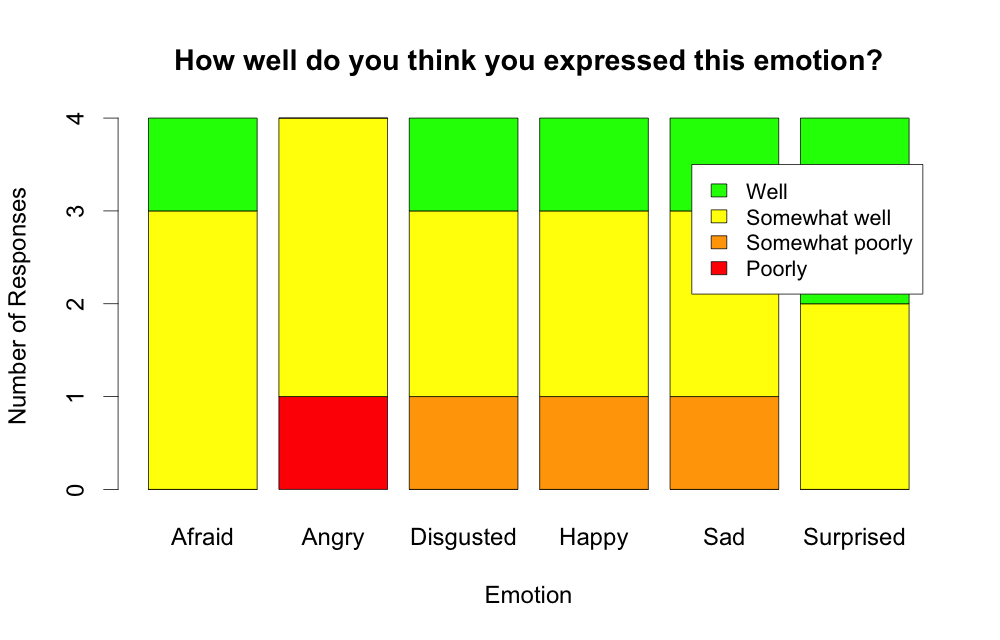
\includegraphics[width=0.47\textwidth]{mHIVE-BarPlot} 
%   \caption{Participant ratings of the confidence in their designs}
%   \label{fig:design:bar:plot}
%\end{figure}


%\strongitem{Memory and attention barriers}
\strongitem{More visualization and recording}
%Though the participants were able to create initial designs for sensations, they were unable to develop them.
Part of mHIVE's inability to support tweaking was due to cognitive limitations for both memory and attention.
Participants found it difficult to remember what they had tried before, % and found it difficult 
and to pay attention to the output % sensation 
while simultaneously controlling it. %the device.
%Participants found significant cognitive challenge in remembering what they had tried before
%	\nq{2}{I tried to recreate that but I couldn't create it exactly as it felt the first time}
\nq{3}{There's a lot of variables which, when I'm trying to compare between two configurations\ldots it was hard sometimes to remember what I had tried},
%if I've done something,
%\theme{Tactile Overshadowing, Looping is required}
%Participants unanimously expressed a desire to feel sensations without having to simultaneously control the device, allowing participants to focus on the sensations they were feeling. This was achieved either by using the recording functionality or the interviewer control mHIVE:
	\nq{1}{I definitely liked being able to feel a stimulus without having to implement it, you know, it allows me to focus more on what it feels like}.
%%	\nq{3}{it's bit hard to do, like I'm trying to go for what I'm imagining, it's hard to do it and feel it at the same time I guess?}
%%	\nq{2}{I tried to recreate that but I couldn't create it exactly as it felt the first time}
%%One thing all participants mentioned was a difficulty remembering what they had previously created or developed. This was partially alleviated by recording, but a desire for more history was deemed important:
%	\nq{3}{It was neat when I could play it back and be like, what did I do and I could see, oh I did that\ldots
%	%and then being able to see where it was was very useful, cuz that helped me in, in what I wanted to be able to kind of replay, like 
%	oh I remember doing something that might work in this situation}.

%This was especially true when the participants noticed a delay between touching the tablet screen and the haptuators activating.  \sq{Feels like there's a delay}, \nq{2}{If I don't look at your finger, I don't see the asynchrony}.

%\strongitem{More visualization and recording}
Participants suggested that although % though 
visualization and recording features helped somewhat %a little 
to overcome these limitations, more was needed. % they needed to be improved.
%All participants requested a further emphasis on recording through repetition or looping.
%This was intended to both aid memory and allow participants to focus on the sensation without worrying about controlling the device.
All  requested greater emphasis on recording through repetition or looping, both to aid memory and allow for focus on the sensation independent of device control. 

%
%\km{SLC***: simultaneous compose/review bad; fluid mode shifting good?} % KM: just struck me: does this undermine the key starting premise that we should be able to perceive the design output AS we create it? In fact, we're finding that this is cognitively too hard. Is it the same for music? Maybe what we have learned is that you need a little space, but not much; and perhaps it is more important that the cognitive effort and time elapsed in moving between composition and review is very streamlined - i.e. you do them separately, but the movement between modes must be extremely fluid.


Allowing persistent, modifiable sensations and alternative visualizations could also help participants overcome these limitations.
%These cognitive challenges were exacerbated when developing more complex sensations.
%mHIVE's recording and visualization capabilities were critical for dealing with these challenges during the design process.
%The visual trail on the main frequency-amplitude screen was especially well received, both aesthetically and for practical use.
%Recorded sensations were important for developing more complicated sensations and augmenting participant memory:
%\nq{2}{The recording functionality I would use for designing more complicated icons that I want to feel different and pleasant}.
%, sometimes goofy or funny
%\nq{2}{Feels great, I love the GUI, a lot},
%\nq{2}{I like the visualization, I like that the history is visible}.
%However, the recording and visualization features are simply not enough as is.
	\nq{3}{The recording records what I do, but it'd be nice to have it repeat stuff},
%This was sometimes meant to mean repeating a single note (P3 quote TODO) but also lead to suggestions of direct manipulation and history:
%Additional visualization was suggested in different forms, improving the trail and seeing the output signal.
%\nq{3}{I almost wanted to be able to see an actual output of the electrical signals\ldots I was having a hard time doing it just by feeling, I would've liked to be able to see it},
%\strongitem{Modification}
%Participants unanimously wanted to modify sensations that had been created.
	\nq{1}{It might conceivably be nice to be able to, you know, draw a curve, draw a pattern, draw like you would in paint, and then be able to manipulate it, replay it, move the points, see what happens}.
%\nq{2}{What I would like to do is, to record something like this, or say go from here to here with the same pace, a constant speed, and then say, okay now, add some acceleration or deceleration to this movement},
%	\nq{3}{Once I zeroed in on something that I thought was close, I almost want to be able to record that spot and then like, tweak it}.

%These design directions may push towards previous tools, like the vibrotactile score \cite{Lee2012, Lee2009}.
%However, it is important to keep some of the novelties created by the haptic instrument, whether as a development paradigm or an interaction technique.
%Rather, combining the two paradigms of editing and collaborative real-time control, either in a single tool or as steps in the design process, might be the best direction. 
%% \kmEdit{slc}
%% Trying to decide if you mean tight integration between two tools in a design-process kind of way; or integrating them within a single tool? 
%	\sq{If you could, transfer this to a desktop computer and then play with it on the desktop computer},
%	\nq{2}{Definitely those options would bloat the interface\ldots so you don't want to sacrifice the good interface that you have for a lot of functionality that a lot of people don't want}.

%One thing all the participants wanted was for recorded sensations to loop and be modifiable:

%	\nq{1}{The other thing was, I think a little bit difficult,is\ldots
%	%you know there was one or two instances where I wanted to, um, you know
%	if I wanted to change something over the course of recording, you know if I wanted to change the waveform as part of the same recording that it was, you know, I couldn't do that quickly}





%%\theme{Visualizations are important}
%%The answer to 
%%Visualizations were critical  \textbf{TODO}
%%The amplitude-frequency view and its graphical trail was well received, especially by P2: \q{Feels great, I love the GUI, a lot}, \q{I like the visualization, I like that the history is visible}.

%P1 enjoyed the visualizations, but wasn't sure if it was useful at first: \q{at first I wasn't sure whether I liked the trails or not, and I still don't think they actually do me any good, but I like them just, aesthetically\ldots you know what maybe they do, because they allow me to, uh, think visually about uh, about what I'm doing and they also allow me to, uh, reproduce and tweak, um, a stimulus.}
%% You know I, I can do this, the output's kind of like that, but I, I, and so the, it's easy to tell I'm doing the same thing again, it's also easy to tell how I'm changing}

%P3 actually wanted more visualization, particularly of the outputted electrical signal: \q{I almost wanted to be able to, um, see like an actual, like, output of the, electrical signals, so that I could really map\ldots I was having a hard time doing it just by feeling, I would've liked to be able to see it.}





%Further comments suggested that the design process was split into two tasks: generation of ideas and tweaking.
%The recording function was a first step towards stronger design capabilities, but tweaking required more power.
%Participants wanted to modify existing stimuli, such as adjusting speed or length of a sensation, automatically loop or sequence sensations, and manually enter values for the parameters (e.g., ADSR).

%%	\nq{1}{but it- it seems like a weird tool cuz it's so constrained, right, but when I think about it as, oh I'm just defining a single tone, um, then it makes sense, and it seems like a handy thing to have.}

%	


%Though participants wanted additional functionality to support tweaking, they thought it might be best implemented in a second tool or mode:
%	
%	\nq{4}{
%	%Either that or if you just have a, selecting, buttons like this, you wouldn't need this free form control, and
%	you'd obviously need two interfaces, one with this freeform, uh digital entry and another one you can just program in what you want.}


%\theme{Hard to remember what was tried}
%Part of mHIVE's inability to support tweaking was due to a poor support of sensation history.


%	\nq{3}{it was neat when I could play it back and be like, what did I do and I could see, oh I did that, and then being able to see where it was was very useful, cuz that helped me in, in what I wanted to be able to kind of replay, like oh I remember doing something that might in this situation.}

%However, the mHIVE's recording and visualization features are not enough.
%Participants were lost in the complexity, and indicated a desire for looping or direct manipulation that would allow changes to existing sensations.
%This is an important direction for improvement, because could help challenges for both attention (by allowing participants to focus entirely on the looping sensation) and memory (by allowing modifications instead of requiring a sensation to be redrawn each time).

%	\nq{1}{it might conceivably be nice to be able to, you know, draw a curve, draw a pattern, draw like you would in paint, and then be able to manipulate it, replay it, move the points, see what happens.}
%	
%	\nq{1}{The other thing was, I think a little bit difficult,is you know there was one or two instances where I wanted to, um, you know if I wanted to change something over the course of recording, you know if I wanted to change the waveform as part of the same recording that it was, you know, I couldn't do that quickly,}

%	\nq{3}{the recording records what I do, but it'd be nice to have it repeat stuff like that}
%	
%These design directions may push towards previous tools, like the vibrotactile score (cite).
%However, it is important to keep some of the novelties created by the haptic instrument, whether as a development paradigm or an interaction technique.
%Rather, combining the two paradigms of editing and collaborative real-time control might be the best direction.

%	\nq{2}{If you could, transfer this to a computer, to a desktop computer and then play with it on the desktop computer},
%	\sq{definitely those options would bloat the, interface so, somehow you want to, um, not go that way, as well, so you don't want to sacrifice the good interface that you have for a lot of functionality that a lot of people don't want.}

%One thing all the participants wanted was for recorded sensations to loop and be modifiable:

%	\nq{1}{The other thing was, I think a little bit difficult,is\ldots
%	%you know there was one or two instances where I wanted to, um, you know
%	if I wanted to change something over the course of recording, you know if I wanted to change the waveform as part of the same recording that it was, you know, I couldn't do that quickly}


\theme{A Difficult Language}
% Unfortunately, We report here on some of the emerging trends.
Our study was too small to analyze language patterns in detail, but exposes emerging trends.

%\theme{ADSR and low-frequencies are pleasant, constant high-frequencies are unpleasant}

\strongitem{Pleasantness, ADSR, and frequency}
Participants often started with a statement of like or dislike rather than a description.
% frequently first stated whether they liked or disliked a sensation, rather than describing  the sensations.
Pleasant sensations often involved the
%Participants used a variety of approaches to describing the sensations that they felt.
%It was sometimes difficult to find appropriate words.
%One of the most common exclamations was whether a participant liked or disliked a sensation.
%This was sometimes more immediate and natural than adjectives.
ramp-in and ramp-out (``echo" or ``ringing") of the ADSR envelope, or lower-frequency sensations.
Longer, higher frequency without ramp-in and ramp-out were less pleasant.
% were especially tied to creating a pleasant sensation.
%In keeping with the literature about touch being connected to affect or \ldots (cite, ask Hasti for refs), participants frequently and readily expressed when they liked a sensation:
	\nq{1}{I don't know how else to describe it, I kinda like it},
%	\nq{3}{I like that}
%This was especially true when introduced to the ADSR envelope:
%	\nq{1}{Oh that's cool, it definitely allows you to change, um, uh, feel, the� niceness? of the tone}, \sq{kinda like that with the square wave, I didn't like the square wave before}	
	\sq{Yeah, this [ADSR] seems natural, somehow}, \nq{2}{It feels unnatural to kill the echo right away},
%	\nq{3}{(TODO)}
%While exploring the device, participants tended to divide frequency and amplitude into two or three discrete values: low, high, and sometimes medium.
%Initially, participants tended to press and hold, rather than tap rhythms (often until prompted by R1).
%The labeled axes divided the main frequency-amplitude interface into quadrants, and afforded this discretization.
%The lower-frequency section (approx. 0-20Hz) provided some variation, when the individual pulses of the actuator could be felt.
%Lower-frequency sensations were often pleasant, while a continuous, high-frequency (150-180Hz) sensation was unpleasant.
%	\nq{2}{I like the sensation of the very low frequency, it's very warm},
	\nq{3}{I like this [low-frequency] sensation cuz to me it feels a lot like purring}.
%Correspondingly, all participants agreed that a sustained high-frequency (right-half of the view, or over 90Hz) was unpleaseant or associated with negative emotions:
%	\nq{1}{I find there's negative emotions I would also associate with high frequencies, definitely anger is a high frequency thing},
%	\nq{2}{I feel like the high frequency one can become disturbing, if the use is prolonged}.
%	\nq{3}{sad was hard, because, I feel like, the high vibration frequencies are agitating so they're okay with negative emotions, and it's a little bit harder at the high speeds to get something that's happier feeling but low, I feel like on this was kind of hard}


%\nq{2}{I'm trying the extreme points first. And middle points.}


\strongitem{Waveform}
%\theme{Waveforms feel qualitatively different, and might gave sensations of frequency}
Participants all noticed differences between waveforms, but were often challenged in expressing them
% although it was often challenging to express the difference
(P4 
%described the differences with 
used the musical term ``timbre").
Square waves in particular were distinct, with a greater range and stronger affinity to mechanical sensations.
	\nq{1}{It's interesting, they feel more different than I thought they would},
	\nq{2}{If you want to make something feel like a motorcycle, you would definitely need square wave}.
%The different waveforms also compounded with frequency -- some waveforms felt like they had higher frequency content in them than others.
%%	\nq{3}{oh not as maybe nice as sine}, \sq{I like it better with the triangle.}
%%The different waveforms felt like they had different frequency content. In some cases this was minor or questioned:
%	\nq{1}{The corners must excite other vibration modes, there's definitely more high frequency information there},
%	\sq{Maybe a sine wave with a frequency of f is equal as a square wave with frequency of 2f}, \nq{2}{Saw feels the highest, then sine, then square and then triangle}.
%	P3 noticed and considered frequency differences between the waveforms, but then decided they weren't salient enough.
%	\nq{3}{I don't think the frequencies are changing, I think it's just the style}.
%%\theme{Common descriptors included sonic, tactile, and abstract-affective metaphors}

\strongitem{Aural/haptic metaphors drawn from previous experience}
For the most part, participants used concrete examples and direct analogies to describe sensations, often drawn from their previous experiences.
One stand-out strategy employed by all participants %to describe sensations 
was % the use of 
onomatopoeias: \nq{1\&4}{beeooo}, \nq{1}{vroom}, \sq{bsheeeooo}, \sq{boom}, \sq{neeeaa}, \nq{2}{mmmMMMmmm}, \sq{pa pa pa pa}, \sq{tum tum tum tum}, \nq{3}{tumba tumba tumba tumba}; \nq{4}{upward arpeggio, like, (singing with hand gestures) na na na naaa}.
Other sound-based metaphors were very common, including hum, buzz, whistle, rumble (P1); bell (P1, P2); squeaky, creak (P2); or thumpy (P3).
%Part of this was influenced, for P1, by hearing the haptuators (especially at higher frequencies).
%In response, R1 reduced the volume for P2-4.
%Audio metaphors were still used; even the word ``sounds" was used instead of ``feels": \nq{4}{Triangle, sounds nicer, er feels nicer (laughing)}.
%This may be isolated to vibrotactile output, and might not generalize to force-feedback output.
Still other descriptors were directly haptic in nature:
rough, flat (P1);
sharp, round, ticklish (P2);
sharp, smooth, cat pawing (P3);
impatient foot tapping (P4).


%\strongitem{Previous experiences}
%Participants especially drew on their previous experience for direct haptic metaphors.
%P3, a pet-owner, used several biological metaphors related to her background:
%	\nq{3}{%As you know, 
%A lot of my experience developing haptic outputs has been trying to develop biological metaphors for haptic outputs, so I think in part, I'm just used to thinking about these kinds of things, the kind of biological, twist to them?}.
%%	 Or more natural twist, um, I think that's most of it}
%Biological metaphors were also used by P2 (\q{This feels like someone throwing up (laughing)} ) and P1 (\q{This to me feels like the device is breathing, kind of like a tactile equivalent to the little light on the front of a MacBook}), but were more isolated.

%
%Cars and motors were another common direct metaphor, particularly at low frequencies.
%%This was also related previous experience: P2 mentioned that he pays a lot of attention to car engines, and drives a manual car.
%This was also related to previous experience: P2 mentioned that he pays a lot of attention to car engines, and drives a manual (stick-shift) car.
%This might explain why it was so commonly mentioned, as a car engine is a common experience.
%	\nq{2}{It feels like, feeling cars passing by, as if you can touch something on the side of the road\ldots like a lamp post that vibrates with cars},
%	\nq{3}{Like a car running},
%	\nq{4}{Sort of a revving sound, like revving an engine}.
	
%\strongitem{Few abstract metaphors}
%Although most descriptors were concrete, some more abstract adjectives were used.
%Abstract terms were typically structural in nature, typically involving the control parameters (amplitude, frequency).
%Other terms were used, some in relation to an overall strength (intense, dainty, has presence), some affective in nature (goofy, serious, playful).
%We did not encounter enough of these terms to notice trends.

%More colourful abstract descriptors were still related to the control parameters (intense, dainty, has strong, has presence), or affective during the design task.


%%%%%%%%%%%%%%%%%%
%
% SECTION: Discussion
% 
%%%%%%%%%%%%%%%%%%
\section{Discussion}
\osC{TODO: modify and link this discussion to other chapters, once they are better established.}
Here we interpret these themes to draw implications for haptic design tools, and compare to research on the language of haptics.
We then reflect upon our methodology and limitations.

%
% Discussion: Design Tools
%
\subsection{Design Tools}

mHIVE was able to achieve the two main goals of a haptic instrument, facilitating both exploration and collaboration.
Participants were clearly able to explore the different low-level parameters, and encountered serendipitous or unexpected sensations through improvisation.
mHIVE created a shared experience that facilitated communication between R1 and the participants.
%The dual outputs created a shared context, demonstrated by deictic phrases where the additional context of the vibrotactile sensation was required to make sense of the statement.
%Direct expression of haptic ideas without names occurred: Participants referred to stimuli as ``this" or ``that," meaning that participants did not need to give names to sensations to discuss them.
%The device was sometimes used as a means of almost gestural expression inserted into conversation.
We can thus conclude that haptic instruments are a promising new tool in a haptic designer's arsenal, with a first, successful implementation in mHIVE.

However, the second theme shows that serendipity and communication are only part of the equation.
mHIVE does not serve as a general editor of haptic sensations.
In particular, participants found their attention split when controlling the device and feeling the sensation; perhaps the real-time control should allow for a rapid, but not instantaneous, switch in focus between control and perception.
%Though mHIVE was successful in its goals, its present form does not also serve as an editor.
More generally, participants were unable to tweak sensations because there was insufficient support for comparing ideas or evolving an existing idea.
%for previous sensations, memory and attention. difficulty of remembering what had been explored before, and the difficulty of paying attention to the sensation perceptually while creating it.

% This difficulty is unsurprising, 
In hindsight, this general difficulty is understandable given the broader context of the musical instrument analogy we used for inspiration.
%The other two problems are cognitive-perceptual barriers that must be addressed when considering the entire work flow for haptic sensations.
Musical instruments are not used to write songs on their own, but % need to be 
combined with notation or recording media.
% This
A similar combination of a haptic instrument and recording might be described more succinctly as %with
 a \emph{haptic sketchpad}.
Sketching is critical in design because it allows for the evolution of an idea through multiple sketches, as well as criticisms, comparisons, and modifications \cite{Cross2011}.
%By adopting a more visual, modifiable tool, we can support tweaking.
Emphasizing a history feature that supports multiple versions of sketches, the user could develop an idea as if with a multiple pages in a sketchbook.
Haptic sketching in hardware has already been shown to be %very 
effective \cite{Moussette2011}.  %; we plan to explore more visual metaphors with future iterations.
As well, a visual metaphor resonates with the desire for more effective visualization.
%, so a software perspective might be promising
%A haptic sketchpad would make heavier use of visual working memory to offset the noted perceptual-cognitive challenges with .
%Of course, effective visualizations are challenging, and are left to future work.

Ultimately, haptic instruments may be most useful as one element
% might be useful as one type of tool  % 
in a suite, or component of a more general tool.
% As part of a suite of tools, mHIVE or other 
A haptic instrument could complement % work together with 
a graphical editing tool that does support tweaking, such as the vibrotactile score \cite{Lee2012,Lee2009} or the hapticon editor \cite{Enriquez2003}.
%This path mirrors musical development directly, and so more inspiration might be from digital audio tools.
As part of a more comprehensive tool, mHIVE could be improved to reduce cognitive barriers to memory and attention.
Alternatively, we could add functionality to mHIVE to support looping, visualization, and direct manipulation of the sensations within the tool.
We will explore these options as we iterate on mHIVE's design in future work.

%This latter approach might suggest that musical instrument metaphor needs to be used more broadly.



%
% Discussion: Language
%
\subsection{Language}

Our preliminary results for language are compatible with the literature,
%providing inductive, empirical evidence
supporting previous work.
% The
Participants' readiness to say whether a sensation was pleasant or not supports the 
% current consensus % KM: I wouldn' say it's a consensus yet.
view that touch is affective in nature, and that knowing what one likes or doesn't like is a primary function of touch \cite{Jansson-Boyd2011}.
ADSR pleasantness and high-frequency unpleasantness are both consistent with the literature: Zheng and Morell note that ramped signals influenced affect more positively than step signals, and 3s high-frequency sensations were annoying or agitating \cite{Zheng2012}.
The heavy use of onomatopoeias is reminiscent of Watanabe \emph{et al}.'s work with static materials \cite{JunjiWatanabeTomohikoHayakawaShigeruMatsuiArisaKanoYuichiroShimizu2012}.
%, albeit in English rather than Japanese.
However, in our study, onomatopoeias were often used to express dynamic sensations (beeeooo being a gradual decrease in amplitude and frequency), which might be a useful direction for future work.

%Participants tended to split the frequency space into either low/high, or low/middle/high frequency regions.
%Though this lends support to the low/high frequency split found in the literature \cite{Obrist2013,Zheng2012}, participants did use dynamic changes in both frequency and amplitude, again suggesting that dynamism is an important direction for future work.

%Because of the consistency with the literature, our other discovered language themes might be appropriate for future areas of research.
%Personal experience and direct analogies might make promising starting points for designers, by focusing on making tactile sensations based on common experiences.
%As the language of touch is developed, we can even consider using higher-level parameters, such as changing the ``roughness" or ``pleasantness" of a sensation, rather than frequency or amplitude.
%This will require more analysis, and is left to future work.
%However, we can say that the parameters chosen for mHIVE seem to be effective for controlling vibrotactile stimuli at this point in time.

%
% Discussion: Methodology and Limitations
%
\subsection{Methodology and Limitations}

Although phenomenology is uncommon in the haptics community (excluding \cite{Obrist2013}), we found it to be an effective way to empirically examine the subjective experience of using mHIVE.
%This was especially true when examining the more nebulous concepts of affect, rather than perceptual thresholds found in psychophysics studies.
Because the community is still developing processes and tasks for haptic design, qualitative studies seem to be an especially appropriate way to tackle these problems.
Once we have further defined haptic design, we can then move to more task-based, experimental methods.
%Of course, these will hopefully be triangulated with controlled, statistically rigorous studies.

Our study was a first round of feedback to inform our next iteration, and has limitations.
%There are limitations to this study that we must mention.
First, our participant pool is (intentionally) small,
%Four participants was sufficient for the rich data we needed at this stage in the design process.
and participants were all collected through our professional network, as people with haptic design experience are rare.
As we continue to tackle the problem of haptic design, we hope to seek out a larger and more diverse pool of participants, and %understand different aspects of the problem through different methods.
%In particular, we hope to
explore more realistic design tasks. %with future work as we iterate upon our tools.



%%%%%%%%%%%%%%%%%%
%
% SECTION: Discussion
% 
%%%%%%%%%%%%%%%%%%
\section{Discussion}
Ultimately,
mHIVE was able to achieve the two main goals of a haptic instrument, facilitating both exploration and collaboration, which showed value in real-time exploration and a shared output context.
mHIVE also had limitations - participants could not edit sensations and found it difficult to keep track of multiple sensations.
This is understandable given the broader context of the musical instrument analogy we used for inspiration.
Musical instruments are not used to write songs on their own, but % need to be 
combined with notation or recording media.
There may be no silver bullet with haptic design tools, with haptic instruments solving a particular set of processes (quick, easy ideation and communication for experts) but not others (final touches, distribution).
Ultimately, haptic instruments may be most useful as one element
% might be useful as one type of tool  % 
in a suite, or component of a more general tool.
%A designer could keep a haptic instrument to quickly sketch ideas while working with a more heavyweight tool that allows for manipulation of a haptic sensation.
%This could be in an ``exploration mode", or perhaps a portable tool to sketch ideas when not near a haptic editing suite.

We follow-up on these leads in our subsequent design studies.
In \autoref{ch:tactileanimation}, we use a persistent model of a VT sensation for an editor, and confirm the value of real-time feedback while expanding the design palette to include spatial haptics.
In \autoref{ch:macaron}, we attempt to mitigate the difficulty of describing haptics and draw upon examples by using a VT design gallery.




%Participants were clearly able to explore the different low-level parameters, and encountered serendipitous or unexpected sensations through improvisation.
%mHIVE created a shared experience that facilitated communication between R1 and the participants.
%We can thus conclude that haptic instruments are a promising new tool in a haptic designer's arsenal, with a first, successful implementation in mHIVE.

%However, the second theme shows that serendipity and communication are only part of the equation.
%mHIVE does not serve as a general editor of haptic sensations.
%In particular, participants found their attention split when controlling the device and feeling the sensation; perhaps the real-time control should allow for a rapid, but not instantaneous, switch in focus between control and perception.
%More generally, participants were unable to tweak sensations because there was insufficient support for comparing ideas or evolving an existing idea.
%
%
%A similar combination of a haptic instrument and recording might be described more succinctly as %with
% a \emph{haptic sketchpad}.
%Sketching is critical in design because it allows for the evolution of an idea through multiple sketches, as well as criticisms, comparisons, and modifications \cite{Cross2011}.
%%By adopting a more visual, modifiable tool, we can support tweaking.
%Emphasizing a history feature that supports multiple versions of sketches, the user could develop an idea as if with a multiple pages in a sketchbook.
%Haptic sketching in hardware has already been shown to be %very 
%effective \cite{Moussette2011}.  %; we plan to explore more visual metaphors with future iterations.
%As well, a visual metaphor resonates with the desire for more effective visualization.
%%, so a software perspective might be promising
%%A haptic sketchpad would make heavier use of visual working memory to offset the noted perceptual-cognitive challenges with .
%%Of course, effective visualizations are challenging, and are left to future work.

%Ultimately, haptic instruments may be most useful as one element
%% might be useful as one type of tool  % 
%in a suite, or component of a more general tool.
%% As part of a suite of tools, mHIVE or other 
%A haptic instrument could complement % work together with 
%a graphical editing tool that does support tweaking, such as the vibrotactile score \cite{Lee2012,Lee2009} or the hapticon editor \cite{Enriquez2003}.
%%This path mirrors musical development directly, and so more inspiration might be from digital audio tools.
%As part of a more comprehensive tool, mHIVE could be improved to reduce cognitive barriers to memory and attention.
%Alternatively, we could add functionality to mHIVE to support looping, visualization, and direct manipulation of the sensations within the tool.
%Many of these results fed into the next case study, Tactile Animation, which expanded to include space and time as controlled dimensions.


\endinput
